% Coherence Collapse Analysis: The Chronometry of Coherence in Networked Systems
% A formal method for failure mode identification in sociotechnical systems

\documentclass[11pt,a4paper]{article}

% Core packages
\usepackage[utf8]{inputenc}
\usepackage[T1]{fontenc}
\usepackage{amsmath,amssymb,amsthm}
\usepackage{mathtools}
\usepackage{graphicx}
\usepackage{xcolor}
\usepackage{hyperref}
\usepackage{cleveref}
\usepackage{booktabs}
\usepackage{array}
\usepackage{float}
\usepackage{enumitem}
\usepackage{tikz}
\usetikzlibrary{shapes,arrows,positioning,calc}
% Algorithm formatting removed - using enumitem instead
\usepackage[margin=1in]{geometry}
\setlength{\emergencystretch}{3em}

% Theorem environments
\theoremstyle{definition}
\newtheorem{definition}{Definition}[section]
\newtheorem{theorem}{Theorem}[section]
\newtheorem{lemma}[theorem]{Lemma}
\newtheorem{corollary}[theorem]{Corollary}
\newtheorem{proposition}[theorem]{Proposition}
\newtheorem{axiom}{Axiom}

\theoremstyle{remark}
\newtheorem{remark}{Remark}[section]
\newtheorem{example}{Example}[section]

% Custom commands
\newcommand{\keff}{k_{\text{eff}}}
\newcommand{\Kreq}{K_{\text{req}}}
\newcommand{\Ttruth}{T_{\text{truth}}}
\newcommand{\Tentropy}{T_{\text{entropy}}}
\newcommand{\Tcapture}{T_{\text{capture}}}
\newcommand{\Teff}{T_{\text{eff}}}
\newcommand{\rhocrit}{\rho_{\text{crit}}}
\newcommand{\sigmin}{\sigma_{\text{min}}}
\newcommand{\R}{\mathbb{R}}
\newcommand{\N}{\mathbb{N}}
\newcommand{\E}{\mathbb{E}}
\newcommand{\Prob}{\mathbb{P}}

% Colors for diagrams
\definecolor{chaosblue}{RGB}{52,152,219}
\definecolor{healthygreen}{RGB}{46,204,113}
\definecolor{rigidityred}{RGB}{231,76,60}
\definecolor{singularitypurple}{RGB}{155,89,182}

% Hyperref setup
\hypersetup{
    colorlinks=true,
    linkcolor=blue!60!black,
    citecolor=green!50!black,
    urlcolor=blue!70!black
}

\title{\textbf{Coherence Collapse Analysis}\\[0.5em]
\large Correlation-Driven Diversity Loss in Complex Coordinating Systems}

\author{
Eric Moore\\
\texttt{eric@ciris.ai}
}

\date{January 2026}

\begin{document}

\maketitle

\begin{abstract}
We apply the Kish design-effect identity $\keff = k/(1 + \rho(k-1))$ to coordination among partially-correlated constraints in complex systems, showing that the number of effective independent degrees of freedom collapses to unity as the correlation parameter $\rho \to 1$. The identity is a M\"obius transformation in $\rho$ with asymptotic ceiling $\keff \to 1/\rho$ for $k \to \infty$ at fixed $\rho > 0$: increasing nominal constituent count does not restore diversity lost to correlation. We identify a singularity boundary $\Kreq \cdot \rho \geq 1$ separating phase regimes (chaos, healthy, rigidity) and derive three closed-form collapse timescales ($\Ttruth$, $\Tentropy$, $\Tcapture$), together with a stability criterion $\alpha/k \geq d$. These are algebraic results, formalized and machine-verified in Lean 4; the Lean development establishes internal consistency and does not bear on external validity.

We describe a 128-sensor GPU-timing strain gauge instrumenting kernel-jitter correlation on an NVIDIA RTX 4090, and report its characterization: fat-tailed (Student-$t$) timing statistics, workload-responsive correlation structure, and the domain over which the equicorrelated precondition the identity assumes actually holds. \textbf{We do not claim the instrument validates the identity.} $\keff = k/(1+\rho(k-1))$ is an identity; it admits no empirical confirmation, and a comparison of values computed from it against values computed from it returns perfect agreement for any formula whatsoever. Establishing that $\rho$ measured in a live system predicts fragility would require an independently observed measure of effective diversity, which this paper does not supply and which remains open.

We prove an information-theoretic barrier (L-01): the class of marginal-preserving deception patterns undetectable by any method operating on marginal distributions alone is \emph{non-empty}. The theorem establishes existence, not measure; the ``$\sim$40\%'' figure appearing in earlier versions follows from a particular illustrative parameterization and is a stated wager, not a result.

CCA is a measurement substrate, not a safety guarantee --- it identifies correlation-driven failure modes; domain experts interpret.

\medskip
\noindent\fbox{\parbox{0.97\textwidth}{\small\textbf{Corrections to v3.} This version corrects eighteen defects in v3 (Zenodo 18217688), several load-bearing: the stability criterion erred in the permissive direction; the cross-domain and institutional validation sections do not support the conclusions drawn from them; and both results previously offered as hardware validation of the $\keff$ identity are identity checks. Defects, evidence, and dispositions are enumerated in the accompanying corrections note, with a machine witness. Readers comparing versions should start there.}}
\end{abstract}

\tableofcontents
\newpage

%==============================================================================
\section{Introduction: The Hypothesis}
%==============================================================================

\subsection{The Core Claim}

We propose that complex coordinating systems---whether biological, chemical, institutional, or artificial---share a common failure mode:

\begin{quote}
\textbf{Correlation accumulation drives effective diversity toward unity, rendering systems fragile to perturbation regardless of nominal scale.}
\end{quote}

This claim is formalized through the \textit{effective constraint count}:
\begin{equation}
\keff = \frac{k}{1 + \rho(k-1)}
\end{equation}
where $k$ is the number of constraints (rules, precedents, species, cells) and $\rho$ is their average pairwise correlation. As $\rho \to 1$, $\keff \to 1$ regardless of $k$. A system with 1,000 highly correlated constraints has the effective diversity of a system with one.

\subsection{The Evidence}

We applied the variable mapping to three empirical datasets from unrelated domains. Version 3 presented the result as cross-domain validation; that reading is withdrawn, and the corrected status of each row is given below.

\begin{table}[H]
\centering
\small
\begin{tabular}{>{\raggedright}p{0.12\textwidth} >{\raggedright}p{0.24\textwidth} >{\raggedright}p{0.20\textwidth} >{\raggedright\arraybackslash}p{0.28\textwidth}}
\toprule
\textbf{Domain} & \textbf{Dataset} & \textbf{Structural Accuracy} & \textbf{Timing Uncertainty} \\
\midrule
Chemistry & NASA Li-ion (19 cells) & 8.1\% RMSE & Overestimates final SOH by $\sim$8\% \\
Political Science & QoG + Polity V & \textbf{Withdrawn}: 2/5, not 5/5, when scored against a pre-specified outcome & \textbf{Withdrawn}: the ``7.6yr early'' figure is an initialisation artifact (\S\ref{sec:institutional-negative}) \\
Biology & American Gut (2,081 taxa) & Matches AGP norms & FMT dynamics simplified \\
\bottomrule
\end{tabular}
\caption{Domain mapping summary, with v3's institutional row corrected. \textbf{The $\keff$ formula is an identity} --- it computes effective constraints from measured $k$ and $\rho$, and admits no empirical confirmation. These rows record how the mapping behaves in each domain; none of them tests the formula.}
\end{table}

The same mathematics is \emph{applied to} battery cell degradation, institutional data, and microbiome composition. Version 3 read this as evidence of a structural property common to constraint-based systems. It is not: the shared mathematics is a modelling choice applied in three places, and applying one formula to three datasets demonstrates that the formula can be applied, not that it holds. The institutional application is now reported as a negative result (\S\ref{sec:institutional-negative}), and the two remaining rows carry proxy $\rho$ values rather than measured intraclass correlations (Table~\ref{tab:keff-application}).

\subsection{The Implications}

If this failure mode generalizes beyond the three tested domains, it may have broader consequences:

\begin{enumerate}[noitemsep]
    \item \textbf{The failure is invisible}: Systems accumulate correlation while appearing healthy ($k$ grows). The collapse of $\keff$ is not directly observable without measuring $\rho$.

    \item \textbf{The failure tends toward simpler configurations}: Under information-theoretic interpretation, correlated systems require less information to describe than diverse ones. Without active maintenance of diversity, systems drift toward homogeneity. (Note: This is an information-theoretic statement, not a claim about physical thermodynamics.)

    \item \textbf{AI accelerates the failure asymmetrically}: AI systems increase constraint count ($k \uparrow$) and correlation ($\rho \uparrow \uparrow$) simultaneously, while externalizing sustainability costs ($\sigma \downarrow$). This masks diversity collapse behind apparent scale \cite{glickman2024, homogenization2025, pnas_echoes2025}.
\end{enumerate}

As a metaphor (not a probabilistic claim), correlation accumulation shares structural features with proposed ``Great Filter'' mechanisms: it operates invisibly, scales with technological capability, and resists intervention once advanced. This analogy is illustrative, not predictive \cite{shumailov2024, cepr2025}.

\subsection{The Framework}

\textbf{Coherence Collapse Analysis (CCA)} is the formal apparatus for analyzing this failure mode. It synthesizes techniques from:
\begin{itemize}[noitemsep]
    \item Failure Mode and Effects Analysis (FMEA) in safety engineering
    \item Stability analysis in control theory
    \item Phase transition analysis in statistical mechanics
    \item Information-theoretic bounds from detection theory
\end{itemize}

CCA provides:
\begin{enumerate}[noitemsep]
    \item \textbf{Failure modes}: How coherence is lost (deception, entropy, capture)
    \item \textbf{Attractor states}: Where systems tend to drift (chaos vs. rigidity)
    \item \textbf{Intervention windows}: When corrective action remains effective
    \item \textbf{Detection limits}: What can and cannot be observed
\end{enumerate}

\subsection{Scope and Falsifiability}

\begin{table}[H]
\centering
\begin{tabular}{>{\raggedright}p{0.45\textwidth} >{\raggedright\arraybackslash}p{0.45\textwidth}}
\toprule
\textbf{CCA Is} & \textbf{CCA Is Not} \\
\midrule
Structural analysis of failure conditions & Prediction of historical outcomes \\
Identification of phase boundaries & Fortune-telling or prophecy \\
An identity applied across domains & Cross-domain validated mathematics \\
Engineering-style failure analysis & Social physics or psychohistory \\
A measurement substrate & A safety guarantee \\
\bottomrule
\end{tabular}
\caption{Scope boundaries for Coherence Collapse Analysis}
\end{table}

\paragraph{Falsification conditions.}
Version 3 stated three conditions, none of which could fire: that ``the $\keff$ formula fails
in additional domains'' (it is an identity, and cannot fail), that ``systems with high $\rho$
demonstrate sustained resilience'' (absorbed by this paper's own block-structure caveat, which
converts any such observation into confirmation), and that ``correlation accumulation reverses
spontaneously'' (no timescale, magnitude, or measurement procedure given). They are replaced
with conditions carrying an observable, a threshold, and a procedure.

\begin{enumerate}[noitemsep]
    \item \textbf{Effective-count disagreement.} Compute $N_{\text{eff}} = k/\lambda_{\max}$ from the largest eigenvalue of a measured correlation matrix and $\keff = k/(1+\bar\rho(k-1))$ from the same data. These are distinct functionals over distinct inputs. If they diverge by more than $25\%$ across the operating range of $\rho$ on a substrate where the equicorrelated precondition holds (condition 2), the identity is not the right effective-count law for that substrate.
    \item \textbf{Precondition failure in the operating band.} The Kish form assumes exchangeability. If the spectral entropy deficit departs from its closed form by more than $10\%$ anywhere in the band where a deployment actually operates, $\keff$ figures from that band are not licensed. \emph{This condition has already fired on the GPU substrate below $\rho \approx 0.04$}, and bounds the domain of every $\keff$ value reported here.
    \item \textbf{No two-sided corridor.} Measure fragility across a $\rho$ range spanning both corridor edges on any substrate. If fragility is monotone in $\rho$ rather than U-shaped --- in particular if it does not rise again above the upper edge --- the corridor claim fails for that substrate. \emph{This is currently untested}: the F-series measured a maximum $\rho$ of $0.171$ against a stated rigidity edge of $0.43$.
    \item \textbf{Volume decay under correlation.} The decay law $V(k) = V_0 e^{-\lambda \keff}$ predicts a specific effective count from measured volume reduction. If simulated or measured decay implies an effective count differing from $\keff$ by more than a factor of $1.5$, the law is wrong. \emph{This condition has already fired}: the implied count exceeds $\keff$ by $1.9\times$ to $4.1\times$ at $\rho = 0.5$, growing with $k$ (\S\ref{sec:outstanding-validation}).
\end{enumerate}

Two of the four have fired against the framework and are reported as such. A condition that
cannot fire is not a falsification condition, and the three carried in version 3 are withdrawn
rather than reworded.

\subsection{Contributions}

\paragraph{Analytic results.}
\begin{enumerate}
    \item The \textbf{M\"obius structure} of the effective-count map: $\keff$ is strictly monotone decreasing in $\rho$ and saturates at $1/\rho$ as $k \to \infty$ (\S\ref{sec:mobius}). Scale cannot restore diversity that correlation has already collapsed --- at $\rho = 0.1$ the ceiling is 10 effective constraints, at $\rho = 0.5$ it is 2, however many are added. This is substrate-independent and requires no calibration.

    \item A \textbf{stability condition} $\alpha/k \geq d$ separating growing from decaying systems, with the corollary that constant-generation systems are eventually unstable for any decay rate.

    \item Derivation of \textbf{three collapse timescales} ($\Ttruth$, $\Tentropy$, $\Tcapture$) in closed form, and a singularity boundary $\Kreq \cdot \rho \geq 1$ beyond which added constraints cannot reduce incoherence.

    \item A \textbf{chaos--rigidity phase decomposition} and the corridor between them. The chaos arm is measured on the GPU substrate; the rigidity arm is not (Remark~\ref{rem:corridor-arm}).

    \item An information-theoretic \textbf{existence result} (L-01): the class of marginal-preserving incoherence patterns undetectable from marginals alone is non-empty. Existence only --- the theorem gives no measure over that class.

    \item Formal verification of the algebraic results in \textbf{Lean 4}, establishing internal consistency and, as \S\ref{sec:formal-verification} states, nothing about external validity.
\end{enumerate}

\paragraph{Instrument and measurements.}
\begin{enumerate}[resume]
    \item A \textbf{128-sensor GPU-timing strain gauge}, characterized: fat-tailed (Student-$t$) timing statistics, workload-responsive correlation structure, first measurement of correlation propagation velocity ($0.5$ m/s), and a bounded domain over which the equicorrelated precondition the identity assumes actually holds (Exp 117: within $0.8\%$ at $\rho = 0.394$, diverging to $70.8\%$ at $\rho \approx 0.03$).

    \item A \textbf{measurement protocol} for correlation on this class of instrument, derived from a pre-registered replication: a shuffle null (at $n = 30$ samples the null's 95th percentile is $\rho \approx 0.15$), repeated trials with intervals rather than single draws, and rejection of the first measurement after idle. Applying it withdrew one of this paper's own headline results.

    \item An \textbf{open-source implementation} --- Python modules, Lean proofs, simulation scripts, pre-registrations, and the machine witness for every algebraic correction in this version (\texttt{github.com/CIRISAI/RATCHET}).
\end{enumerate}

\paragraph{What this version does not contribute.}
Version 3 of this paper claimed cross-domain empirical validation of the $\keff$ formula and hardware confirmation of its central mathematical claim. \textbf{Both are withdrawn.} $\keff$ is an identity: it admits no empirical confirmation, and the two results previously offered as confirming it computed the identity and compared it against itself. The institutional application does not test $\keff$ at all and is reported here as a negative result (\S\ref{sec:institutional-negative}). Eighteen defects are enumerated with evidence and dispositions in the accompanying corrections note; the two that resist repair --- the $\keff$ substitution in Theorem~\ref{thm:volume-decay}, and the deceptive/honest asymmetry --- are stated as open in \S\ref{sec:outstanding-validation} with measurements of how far each fails.

\subsection{Interpretation Guardrails}

To prevent misreading, we state explicitly what CCA does \textbf{not} claim:

\begin{itemize}[noitemsep]
    \item \textbf{No inevitability}: Correlation accumulation is a tendency, not a fate. Systems can and do maintain diversity through active intervention.
    \item \textbf{No timeline predictions}: CCA identifies \textit{structural fragility}, not when collapse will occur. Version 3 cited a ``7.6-year timing error'' here as illustrating the limitation; that figure is itself withdrawn as an initialisation artifact (\S\ref{sec:institutional-negative}), and the limitation stands without it --- no lead-time claim in this paper survives comparison against a null that fires at $t_0$.
    \item \textbf{No macro-outcome claims}: We do not predict civilizational collapse, AI doom scenarios, or specific historical events. CCA is engineering risk analysis, not prophecy.
    \item \textbf{No causal claim}: CCA does not claim correlation \textit{causes} collapse---only that high correlation is a sufficient structural bottleneck for fragility, regardless of underlying mechanism (see F4: common cause confirmation in Section~\ref{sec:gpu-validation}).
    \item \textbf{``Great Filter'' is metaphorical}: The term is used as an illustrative analogy for correlation-driven failure, not as a probabilistic claim about the Fermi paradox.
\end{itemize}

\noindent The framework's value lies in making hidden fragility \textit{legible}---identifying when systems have drifted into dangerous phase space, not in predicting what happens next.

%==============================================================================
\section{Mathematical Foundations}
%==============================================================================

\subsection{Constraint Geometry}

The foundation of CCA is the observation that system coherence is maintained through \textit{constraints}---rules, precedents, norms, or structural features that limit the space of possible behaviors.

\begin{definition}[Constraint Space]
A \textbf{constraint space} is a tuple $(V, \mathcal{C}, \rho)$ where:
\begin{itemize}[noitemsep]
    \item $V \subseteq \R^n$ is the space of possible system states
    \item $\mathcal{C} = \{C_1, \ldots, C_k\}$ is a set of constraint halfspaces
    \item $\rho: \mathcal{C} \times \mathcal{C} \to [0,1]$ is the pairwise correlation function
\end{itemize}
\end{definition}

The \textit{feasible region} is the intersection $\bigcap_{i=1}^{k} C_i$, representing states consistent with all constraints. Deceptive or incoherent behaviors correspond to states outside this region.

\begin{definition}[Effective Constraint Count]
Given $k$ constraints with average pairwise correlation $\rho$, the \textbf{effective constraint count} is:
\begin{equation}
\keff = \frac{k}{1 + \rho(k-1)}
\label{eq:keff}
\end{equation}
\end{definition}

\begin{remark}[Statistical Provenance]
This formula is mathematically identical to the \textbf{Kish design effect} for effective sample size in survey statistics, which accounts for autocorrelation in clustered samples. We do not claim novelty for the formula itself---only for its application to constraint-based system analysis. The ``validation'' of $\keff$ across domains confirms that the algebra of effective sample sizes holds when variables are appropriately mapped; it does not establish that such mappings are causally meaningful in all contexts.
\end{remark}

This captures the intuition that correlated constraints provide redundant information:
\begin{itemize}[noitemsep]
    \item When $\rho = 0$ (independent): $\keff = k$
    \item When $\rho \to 1$ (fully correlated): $\keff \to 1$
\end{itemize}

\begin{remark}[M\"obius Structure and Asymptotic Ceiling]
\label{sec:mobius}
For fixed $k$, the map $\rho \mapsto \keff(k, \rho)$ is the M\"obius transformation with coefficients $(a, b, c, d) = (0, k, k-1, 1)$. The partial derivative $\partial \keff / \partial \rho = -k(k-1)/(1 + \rho(k-1))^2 < 0$ for $k > 1$, so $\keff$ is strictly monotone decreasing in $\rho$ on $[0, 1]$. Taking $k \to \infty$ at fixed $\rho > 0$:
\begin{equation*}
\lim_{k \to \infty} \keff(k, \rho) = \lim_{k \to \infty} \frac{k}{1 + \rho(k-1)} = \frac{1}{\rho}.
\end{equation*}
Effective dimensionality saturates at the inverse correlation regardless of nominal constituent count. \textbf{Adding more correlated constituents cannot restore diversity that correlation has already collapsed:} at $\rho = 0.1$ the ceiling is $\keff = 10$; at $\rho = 0.5$ it is $\keff = 2$; at $\rho = 0.9$ it is $\keff \approx 1.11$. This is the algebraic core of the ``scale alone cannot compensate for lost diversity'' claim, and it is independent of any substrate-specific calibration.
\end{remark}

\begin{remark}[Scalar $\rho$ Limitation]
The average pairwise correlation $\rho$ is a scalar summary that can obscure important structure. \textbf{High average $\rho$ does not imply collapse when correlation is modular rather than global.} A system with two independent clusters, each internally correlated, may show high average $\rho$ but retain $\keff = 2$ (the number of independent modules). The E-series experiments (Section~\ref{sec:gpu-validation}) explicitly test for block-diagonal correlation structure. Future work should extend CCA to use correlation tensors that preserve this information.
\end{remark}

\begin{theorem}[Volume Decay]
\label{thm:volume-decay}
Under the following assumptions:
\begin{enumerate}[noitemsep,label=(\alph*)]
    \item Constraints are drawn i.i.d.\ from a distribution over halfspaces with bounded support
    \item The initial feasible region $V_0$ is bounded and convex
    \item Constraint normals have mean zero and covariance $\Sigma$ with $\|\Sigma\| \leq M$ for some $M > 0$
\end{enumerate}
the volume of the feasible region decays exponentially with effective constraints:
\begin{equation}
V(k) = V_0 \cdot e^{-\lambda \cdot \keff} \cdot (1 + O(1/\sqrt{\keff}))
\label{eq:volume_decay}
\end{equation}
where $\lambda > 0$ is the decay constant determined by constraint geometry, and the error term vanishes as $\keff \to \infty$.
\end{theorem}

\begin{proof}[Proof sketch]
Under assumption (a), each independent constraint removes a fraction of the remaining volume. By Gr\"unbaum's theorem on log-concavity of volume under halfspace intersection, the reduction is multiplicative. For $\keff$ effective (non-redundant) constraints, this yields $V(\keff) \approx V_0 \cdot \prod_{i=1}^{\keff} (1 - \delta_i)$ where $\delta_i$ is the fraction removed by constraint $i$. Taking logs and applying the law of large numbers under assumption (c), $\sum \ln(1-\delta_i) \approx -\lambda \cdot \keff$ for some $\lambda$ depending on the constraint distribution. The correlation adjustment ($\keff$ vs $k$) follows from the effective sample size formula: correlated constraints provide redundant information, reducing the effective count by factor $(1 + \rho(k-1))^{-1}$.
\end{proof}

\begin{remark}[Applicability]
The exponential form is an approximation valid when constraints are ``generic'' (no degenerate intersections) and sufficiently numerous. For small $k$ or highly structured constraint sets, empirical validation is required.
\end{remark}

\subsection{The Defense Function}

\begin{definition}[Defense Function]
The \textbf{defense function} $J$ quantifies the computational cost an adversary must pay to maintain incoherent behavior:
\begin{equation}
J = \keff \cdot \lambda \cdot \sigma
\label{eq:defense}
\end{equation}
where:
\begin{itemize}[noitemsep]
    \item $\keff$: Effective scale --- constraint count \textit{after} the correlation discount
    \item $\lambda$: Strictness (constraint strength)
    \item $\sigma$: Sustainability (maintenance capacity)
\end{itemize}
\end{definition}

\begin{remark}[Correction: diversity is carried by $\keff$, not a separate factor]
Version 3 of this paper defined $J = \keff \cdot (1-\rho) \cdot \lambda \cdot \sigma$. That form \textbf{double-counted correlation}: $\keff = k/(1+\rho(k-1))$ already contains the diversity discount, so multiplying by a further $(1-\rho)$ applies it twice and drives $J \to 0$ as $\rho \to 1$. The latter contradicts the single-constraint floor --- a fully correlated system is no safer than \textit{one} constraint, but it is not \textit{worse} than one. The corrected three-factor form above is the one carried by the CIRIS Constitution (CC 6.2.2). Diversity enters $J$ \textbf{only} through $\keff$. See \texttt{CORRECTIONS\_v3.md}.
\end{remark}

\begin{remark}[Definitional Status of $J$]
The defense function $J$ is a \textbf{modeling choice}, not a derived quantity. We do not claim that $J$ is the unique or correct measure of system resilience---only that this particular combination of terms produces useful analysis across multiple domains. Alternative formulations (e.g., weighted products, nonlinear combinations) may be appropriate for specific applications.
\end{remark}

This formulation exhibits a conceptual duality: systems with high defense $J$ against incoherence also tend to have high capacity for coordinated flourishing. High-defense systems are also high-capacity systems.

\begin{proposition}[J-C Duality Interpretation]
Let $C$ denote an abstract ``capacity for coordinated flourishing.'' If we operationalize $C$ as the product of:
\begin{itemize}[noitemsep]
    \item effective coordination channels ($\keff$, which already discounts channels that are not independent),
    \item enforcement strength ($\lambda$), and
    \item resource sustainability ($\sigma$),
\end{itemize}
then $J = C$ by definition. This is not a derived result but a \textbf{definitional choice} that interprets defense and capacity as dual aspects of the same underlying quantity.
\end{proposition}

\begin{remark}
The J-C duality is interpretive rather than mathematical. It asserts that the same structural features that make a system hard to subvert also make it capable of positive coordination. This claim is falsifiable: if empirical systems show high $J$ with low flourishing capacity (or vice versa), the interpretation fails.
\end{remark}

The defense function provides a single scalar that summarizes system health. Its dynamics determine whether the system is growing stronger or collapsing.

\subsection{Stability Condition}

\begin{definition}[Collapse Rate]
The \textbf{collapse rate} is the time derivative of the defense function:
\begin{equation}
R_c = \frac{dJ}{dt}
\end{equation}
\end{definition}

\begin{theorem}[Stability Condition]
\label{thm:stability}
A system is stable if and only if $R_c \geq 0$. Under the simplifying assumption that $\lambda$ is constant, this reduces to:
\begin{equation}
\text{Stable} \iff \frac{\alpha}{k} \geq d
\label{eq:stability}
\end{equation}
where $\alpha = dk/dt$ is the constraint generation rate and $d$ is the sustainability decay rate. Note that the criterion is governed by the \textbf{nominal} count $k$, not by $\keff$.
\end{theorem}

\begin{proof}[Derivation]
From $J = \keff \cdot \lambda \cdot \sigma$, apply the product rule:
\begin{equation}
\frac{dJ}{dt} = \lambda \left[ \frac{d\keff}{dt}\,\sigma + \keff\,\frac{d\sigma}{dt} \right]
\end{equation}

Assume the dominant dynamics are:
\begin{enumerate}[noitemsep,label=(\roman*)]
    \item $\keff$ grows proportionally to new constraints: $d\keff/dt \approx \alpha / (1 + \rho(k-1))$
    \item $\rho$ changes slowly: $d\rho/dt \approx 0$ (quasi-static)
    \item $\sigma$ decays exponentially without input: $d\sigma/dt = -d \cdot \sigma$
\end{enumerate}

Substituting these together with $\keff = k/(1+\rho(k-1))$:
\begin{equation}
R_c \approx \lambda\sigma \left[ \frac{\alpha}{1 + \rho(k-1)} - d \cdot \frac{k}{1 + \rho(k-1)} \right] = \frac{\lambda\sigma\,(\alpha - d\,k)}{1 + \rho(k-1)}
\end{equation}

Since $\lambda, \sigma > 0$ and $1 + \rho(k-1) > 0$ for $\rho \in [0,1]$, $k \geq 1$, the sign of $R_c$ is governed entirely by the factor $(\alpha - dk)$:
\begin{equation}
R_c \geq 0 \iff \alpha \geq d \cdot k \iff \frac{\alpha}{k} \geq d
\end{equation}

The inequality is strict for stability margin.
\end{proof}

\begin{remark}[Correction to v3: the criterion is $\alpha/k$, not $\alpha/\keff$]
Version 3 of this paper stated the criterion as $\alpha/\keff > d$. That does not follow from the derivation above: the common denominator $1+\rho(k-1)$ cancels between the two terms, leaving $(\alpha - dk)$ and hence $\alpha/k \geq d$. Because $\keff \leq k$, the v3 criterion is \textbf{too permissive by exactly $1 + \rho(k-1)$} --- the design-effect factor this paper exists to introduce --- and it errs in the unsafe direction, certifying as stable systems whose defense function is strictly decreasing. For example, at $k=100$, $\rho=0.5$, $d=0.1$, $\alpha=5.099$: the v3 criterion gives $\alpha/\keff = 2.575 > d$ (``stable'') while $dJ/dt < 0$. The correction is independent of the $J$-form correction above: with or without the $(1-\rho)$ factor, the boundary is $\alpha = dk$. Machine witness: \texttt{corrections\_witness.py}; see \texttt{CORRECTIONS\_v3.md}.
\end{remark}

\begin{corollary}[Static Systems Are Doomed]
\label{cor:static}
If $\alpha$ is constant and $k$ grows without bound, the ratio $\alpha/k$ decreases monotonically toward zero. Eventually $\alpha/k < d$, violating stability.
\end{corollary}

\begin{remark}[Why the corollary requires $k$ rather than $\keff$]
This corollary is \textbf{false} under the v3 criterion and is restored only by the correction above. The v3 argument asserted that $k$ growing implies $\keff$ growing, so that $\alpha/\keff$ falls below $d$. But $\keff$ does \textit{not} grow without bound: it saturates at $1/\rho$, so $\alpha/\keff$ converges to $\alpha\rho$ \textit{from above} rather than decaying. Whenever $\alpha\rho > d$ the v3 criterion is never violated, no matter how large $k$ becomes --- at $\rho=0.5$, $d=0.1$, $\alpha=1$ the ratio floors at $0.5$, permanently above $d$. Under the corrected criterion the conclusion holds unconditionally, since $\alpha/k \to 0$ for any fixed $\alpha$. The headline claim survives; it does not survive the reasoning as published.
\end{remark}

\begin{remark}[Dimensional Analysis]
The stability condition is dimensionally consistent: $\alpha$ has units [constraints/time], $k$ is dimensionless, and $d$ has units [1/time]. The ratio $\alpha/k$ gives the rate of constraint generation per existing constraint, which must exceed the decay rate.
\end{remark}

This is a key insight: static systems cannot maintain coherence indefinitely. The stability condition demands continual renewal.

%==============================================================================
\section{Collapse Timelines}
%==============================================================================

CCA identifies three primary collapse modes, each with a characteristic timeline.

\subsection{Time to Truth ($\Ttruth$)}

\begin{definition}[Required Constraints]
Given initial volume $V_0$, target safety threshold $\varepsilon$, and decay constant $\lambda$, the required effective constraints are:
\begin{equation}
\Kreq = \frac{-\ln(\varepsilon/V_0)}{\lambda}
\end{equation}
\end{definition}

\begin{definition}[Critical Correlation]
The \textbf{critical correlation threshold} is:
\begin{equation}
\rhocrit = \frac{1}{\Kreq}
\end{equation}
If $\rho \geq \rhocrit$, the system cannot generate sufficient effective constraints regardless of scale.
\end{definition}

\begin{theorem}[Time to Truth]
The time until incoherent behavior becomes computationally prohibitive is:
\begin{equation}
\Ttruth = \frac{\Kreq(1-\rho)}{\alpha(1 - \Kreq \cdot \rho)}
\label{eq:Ttruth}
\end{equation}
\end{theorem}

\begin{theorem}[Singularity Condition]
When $\Kreq \cdot \rho \geq 1$:
\begin{equation}
\Ttruth \to \infty
\end{equation}
This is the \textbf{rigidity boundary}---an ``echo chamber'' where correlated constraints provide no additional security regardless of scale or time.
\end{theorem}

\subsection{Time to Entropy ($\Tentropy$)}

Systems require ongoing maintenance to prevent entropic decay.

\begin{definition}[Sustainability Dynamics]
The sustainability integral evolves as:
\begin{equation}
\sigma(t) = \sigma_0 \cdot e^{-d \cdot t} + \int_0^t w \cdot S(\tau) \cdot e^{-d(t-\tau)} \, d\tau
\end{equation}
where $S(t)$ is the signal (value production) and $w$ is the weight.
\end{definition}

\begin{theorem}[Time to Entropy]
The time until sustainability falls below the revocation threshold $\sigmin$ is:
\begin{equation}
\Tentropy = \frac{\ln(\sigma/\sigmin)}{d}
\label{eq:Tentropy}
\end{equation}
\end{theorem}

This represents the ``black hole'' failure mode: systems that consume resources without producing value eventually collapse.

\subsection{Time to Capture ($\Tcapture$)}

Distributed systems can be captured through gradual corruption of nodes.

\begin{theorem}[Time to Capture]
For a federation with $n$ nodes, $f$ currently compromised, and capture rate $r_{\text{cap}}$:
\begin{equation}
\Tcapture = \frac{(n/3) - f}{r_{\text{cap}}}
\label{eq:Tcapture}
\end{equation}
where $n/3$ is the Byzantine fault tolerance threshold.
\end{theorem}

\subsection{Effective Collapse Time}

\begin{definition}[Effective Collapse Time]
The \textbf{effective collapse time} is the minimum of all collapse modes:
\begin{equation}
\Teff = \min(\Ttruth, \Tentropy, \Tcapture)
\end{equation}
The \textbf{limiting factor} is whichever timeline is shortest.
\end{definition}

\begin{figure}[H]
\centering
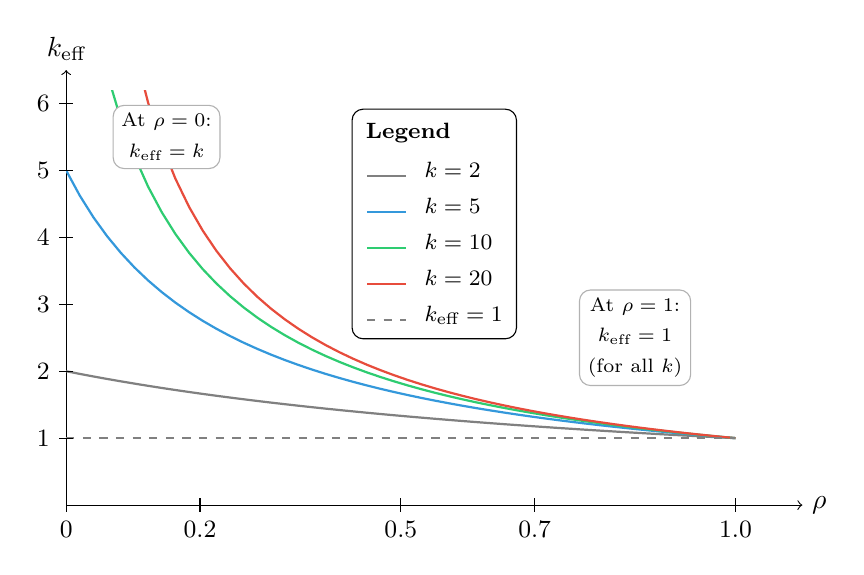
\begin{tikzpicture}[scale=0.85]
    % Axes
    \draw[->] (0,0) -- (11,0) node[right] {$\rho$};
    \draw[->] (0,0) -- (0,6.5) node[above] {$\keff$};

    % Clip region to keep curves within graph bounds
    \begin{scope}
    \clip (0,0) rectangle (10.5,6.2);

    % k_eff curves: k_eff = k / (1 + rho*(k-1))
    % x-axis: rho from 0 to 1 (scaled by 10)
    % y-axis: k_eff directly

    % k = 2
    \draw[thick, gray, domain=0:10, samples=50] plot (\x, {2 / (1 + (\x/10)*(2-1))});

    % k = 5
    \draw[thick, chaosblue, domain=0:10, samples=50] plot (\x, {5 / (1 + (\x/10)*(5-1))});

    % k = 10
    \draw[thick, healthygreen, domain=0:10, samples=50] plot (\x, {10 / (1 + (\x/10)*(10-1))});

    % k = 20
    \draw[thick, rigidityred, domain=0:10, samples=50] plot (\x, {20 / (1 + (\x/10)*(20-1))});

    \end{scope}

    % Horizontal line at k_eff = 1 (rigidity ceiling)
    \draw[dashed, black!50, thick] (0, 1) -- (10, 1);

    % Tick marks - x axis
    \foreach \x/\label in {0/0, 2/0.2, 5/0.5, 7/0.7, 10/1.0} {
        \draw (\x, 0.1) -- (\x, -0.1) node[below] {\small \label};
    }
    % Tick marks - y axis
    \foreach \y in {1, 2, 3, 4, 5, 6} {
        \draw (0.1, \y) -- (-0.1, \y) node[left] {\small \y};
    }

    % Legend box - positioned inside graph bounds
    \node[draw, fill=white, rounded corners, inner sep=5pt, align=left] at (5.5, 4.2) {
        \footnotesize\textbf{Legend}\\[2pt]
        \tikz\draw[thick, gray] (0,0) -- (0.5,0); \footnotesize\ $k = 2$\\[1pt]
        \tikz\draw[thick, chaosblue] (0,0) -- (0.5,0); \footnotesize\ $k = 5$\\[1pt]
        \tikz\draw[thick, healthygreen] (0,0) -- (0.5,0); \footnotesize\ $k = 10$\\[1pt]
        \tikz\draw[thick, rigidityred] (0,0) -- (0.5,0); \footnotesize\ $k = 20$\\[1pt]
        \tikz\draw[dashed, black!50, thick] (0,0) -- (0.5,0); \footnotesize\ $\keff = 1$
    };

    % Annotations
    \node[align=center, fill=white, draw=black!30, rounded corners, inner sep=3pt] at (1.5, 5.5) {
        \scriptsize At $\rho = 0$:\\[-1pt]
        \scriptsize $\keff = k$
    };
    \node[align=center, fill=white, draw=black!30, rounded corners, inner sep=3pt] at (8.5, 2.5) {
        \scriptsize At $\rho = 1$:\\[-1pt]
        \scriptsize $\keff = 1$\\[-1pt]
        \scriptsize (for all $k$)
    };

\end{tikzpicture}
\caption{Effective constraint count $\keff = k/(1 + \rho(k-1))$ as a function of correlation $\rho$. \textbf{Key finding:} Regardless of how many raw constraints $k$ a system accumulates, high correlation ($\rho \to 1$) crushes effective constraints to $\keff = 1$. This is the ``echo chamber'' ceiling---adding more correlated constraints provides no marginal security. \textbf{Conclusion:} Scale alone cannot compensate for lost diversity.}
\label{fig:keff-curves}
\end{figure}

%==============================================================================
\section{Phase Space Analysis}
%==============================================================================

\subsection{The Chaos-Rigidity Spectrum}

Systems can fail in two opposing directions:

\begin{definition}[Chaos]
A system is in a \textbf{chaos trajectory} when:
\begin{itemize}[noitemsep]
    \item Correlation $\rho < 0.2$ (constraints are independent)
    \item Entropy is increasing
    \item Defense function $J$ exhibits high variance
    \item No emergent coordination
\end{itemize}
\end{definition}

\begin{definition}[Rigidity]
A system is in a \textbf{rigidity trajectory} when:
\begin{itemize}[noitemsep]
    \item Correlation $\rho > 0.7$ (echo chamber formation)
    \item $\keff \to 1$ regardless of $k$
    \item Single points of failure dominate
    \item Over-coordination suppresses diversity
\end{itemize}
In CCA, ``rigidity'' denotes an over-coordinated failure regime characterized by constraint redundancy and loss of adaptive capacity. Such systems fail due to Ashby-style requisite variety mismatch: homogeneous constraints cannot absorb heterogeneous perturbations.
\end{definition}

\begin{theorem}[Healthy Corridor]
A system maintains coherence when:
\begin{equation}
0.2 < \rho < \rhocrit \quad \text{and} \quad \frac{\alpha}{k} \geq d
\end{equation}
\end{theorem}

\begin{remark}[Correction to v3]
The second conjunct read $\alpha/\keff > d$ in v3, inheriting the Theorem~\ref{thm:stability} error; it is corrected here to $\alpha/k \geq d$. The corridor bounds on $\rho$ are unaffected. Note separately that the corridor edges are \textbf{substrate-specific} and require per-substrate calibration; the numerical bounds quoted here are GPU-anchored.
\end{remark}

\begin{figure}[H]
\centering
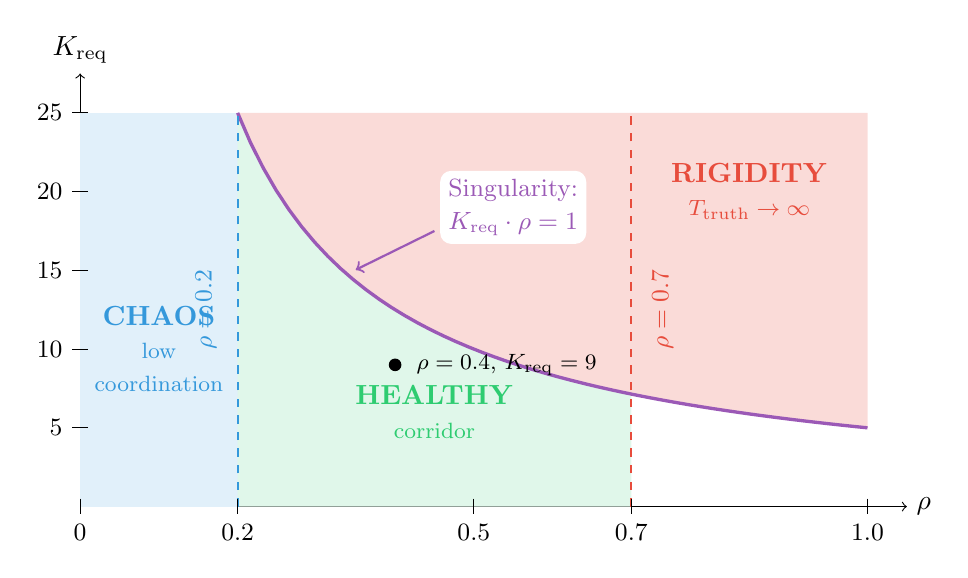
\begin{tikzpicture}[scale=1.0]
    % Axes - x: rho (0 to 1, scaled by 10), y: K_req (0 to 25, scaled by 0.2)
    % At x=2 (rho=0.2): y = 10/2 = 5 (K_req = 25)
    % At x=10 (rho=1.0): y = 10/10 = 1 (K_req = 5)
    \draw[->] (0,0) -- (10.5,0) node[right] {$\rho$};
    \draw[->] (0,0) -- (0,5.5) node[above] {$\Kreq$};

    % Clip to chart bounds
    \begin{scope}
        \clip (0,0) rectangle (10,5);

        % Shade chaos region (rho < 0.2)
        \fill[chaosblue!15] (0,0) rectangle (2,5);

        % Shade the singular region (above the curve)
        \fill[rigidityred!20] (2,5) -- plot[domain=2:10, samples=30] (\x, {10/\x}) -- (10,1) -- (10,5) -- cycle;

        % Shade healthy region (below curve, between chaos and rigidity thresholds)
        \fill[healthygreen!15] (2,0) -- (2,5) -- plot[domain=2:7, samples=30] (\x, {10/\x}) -- (7,0) -- cycle;

        % Singularity curve: K_req * rho = 1, so K_req = 1/rho
        % Scaled: y = 10/x (starts at x=2 where y=5, ends at x=10 where y=1)
        \draw[very thick, singularitypurple, domain=2:10, samples=50] plot (\x, {10/\x});
    \end{scope}

    % Boundary labels
    \draw[dashed, thick, chaosblue] (2,0) -- (2,5);
    \node[chaosblue, rotate=90] at (1.6, 2.5) {\small $\rho = 0.2$};

    \draw[dashed, thick, rigidityred] (7,0) -- (7,5);
    \node[rigidityred, rotate=90] at (7.4, 2.5) {\small $\rho = 0.7$};

    % Region labels
    \node[chaosblue, align=center] at (1, 2) {\textbf{CHAOS}\\{\footnotesize low}\\{\footnotesize coordination}};
    \node[healthygreen, align=center] at (4.5, 1.2) {\textbf{HEALTHY}\\{\footnotesize corridor}};
    \node[rigidityred, align=center] at (8.5, 4) {\textbf{RIGIDITY}\\{\footnotesize $\Ttruth \to \infty$}};

    % Singularity curve label
    \node[singularitypurple, align=left, fill=white, rounded corners, inner sep=3pt] at (5.5, 3.8) {
        \small Singularity:\\
        \small $\Kreq \cdot \rho = 1$
    };

    % Arrow pointing to curve
    \draw[->, singularitypurple, thick] (4.5, 3.5) -- (3.5, {10/3.5 + 0.15});

    % Example point in healthy region
    \fill[black] (4, 1.8) circle (0.08);
    \node[right, align=left] at (4.15, 1.8) {\footnotesize $\rho=0.4$, $\Kreq=9$};

    % Tick marks
    \foreach \x/\label in {0/0, 2/0.2, 5/0.5, 7/0.7, 10/1.0} {
        \draw (\x, 0.1) -- (\x, -0.1) node[below] {\small \label};
    }
    \foreach \y/\label in {1/5, 2/10, 3/15, 4/20, 5/25} {
        \draw (0.1, \y) -- (-0.1, \y) node[left] {\small \label};
    }
\end{tikzpicture}
\caption{Phase space diagram showing the singularity boundary $\Kreq \cdot \rho = 1$ (purple curve). Above this curve, $\Ttruth \to \infty$---the system cannot collapse incoherence regardless of scale or time. The healthy corridor exists between chaos ($\rho < 0.2$) and rigidity ($\rho > 0.7$), below the singularity.}
\label{fig:phase-space}
\end{figure}

\subsection{Classification Algorithm}

\noindent\textbf{Algorithm: Trajectory Classification}

\noindent\textit{Input}: Timeline $\Teff$, measurements $\{(\rho_t, k_{\text{eff},t}, \sigma_t)\}$, thresholds $(\tau_{\text{collapse}}, \rho_{\text{low}}, \rho_{\text{high}}, \delta_\rho)$\\
\textit{Output}: Classification $\in \{\text{HEALTHY}, \text{CHAOS}, \text{RIGIDITY}, \text{COLLAPSE}\}$

\begin{enumerate}[noitemsep]
    \item \textbf{If} $\Teff < \tau_{\text{collapse}}$ \textbf{then return} IMMINENT\_COLLAPSE
    \item $\rho_{\text{recent}} \gets$ most recent $\rho$
    \item $\text{trend}_\rho \gets$ linear regression slope of $\rho$
    \item \textbf{If} $\rho_{\text{recent}} < \rho_{\text{low}}$ \textbf{or} $\text{trend}_\rho < -\delta_\rho$ \textbf{then return} TRENDING\_CHAOS
    \item \textbf{If} $\rho_{\text{recent}} > \rho_{\text{high}}$ \textbf{or} $\text{trend}_\rho > +\delta_\rho$ \textbf{then return} TRENDING\_RIGIDITY
    \item \textbf{Return} HEALTHY
\end{enumerate}

\begin{remark}[Threshold Calibration]
The algorithm requires four domain-specific thresholds:
\begin{itemize}[noitemsep]
    \item $\tau_{\text{collapse}}$: Imminent collapse window (illustrative default: 7 days)
    \item $\rho_{\text{low}}$: Chaos boundary (illustrative default: 0.2)
    \item $\rho_{\text{high}}$: Rigidity boundary (illustrative default: 0.7)
    \item $\delta_\rho$: Trend sensitivity (illustrative default: 0.01/day)
\end{itemize}

These are \textbf{not universal constants}. Calibration procedure:
\begin{enumerate}[noitemsep]
    \item \textbf{Historical fitting}: If collapse events exist in domain history, fit thresholds to maximize classification accuracy on labeled data.
    \item \textbf{Sensitivity analysis}: Vary thresholds $\pm 20\%$ and assess classification stability.
    \item \textbf{Domain expertise}: Adjust based on domain-specific knowledge (e.g., institutional systems may have higher $\rho_{\text{high}}$ than ecological systems).
    \item \textbf{Cross-validation}: Use held-out data to validate threshold choices.
\end{enumerate}
The illustrative defaults are derived from sociotechnical systems with moderate coupling; other domains (biological, chemical, economic) may require substantial recalibration.
\end{remark}

%==============================================================================
\section{Information-Theoretic Limits}
%==============================================================================

\subsection{The L-01 Barrier}

A fundamental result of CCA is that complete detection of incoherence is \textit{provably impossible}.

\begin{theorem}[L-01: Emergent Incoherence Barrier]
There exists a non-empty class of emergent incoherence patterns that are fundamentally undetectable by any statistical analysis method operating on marginal distributions alone.
\end{theorem}

\begin{proof}
Incoherence can be \textit{marginal-preserving}: each component's output distribution matches the coherent distribution when viewed in isolation, while the joint distribution exhibits incoherence. Formally, let $P_{\text{honest}}(X_1, \ldots, X_n)$ be the joint distribution of honest components, and let $P_{\text{deceptive}}$ be a deceptive joint distribution satisfying:
\begin{equation}
\forall i: \quad P_{\text{deceptive}}(X_i) = P_{\text{honest}}(X_i)
\end{equation}
Such distributions exist by construction (e.g., copula coupling with identical marginals). Any detector relying solely on marginal statistics has $I(X_i; \text{label}) = 0$, making detection impossible regardless of sample size.
\end{proof}

\begin{remark}[On the ``40\%'' Estimate]
The specific fraction of undetectable incoherence depends on the generative model for deception strategies. Under the assumption that detection operates via MI amplification with threshold $\varepsilon$, we model detection probability as $P(\text{detect}) = 1 - e^{-\beta\varepsilon}$ where $\beta$ is a sensitivity parameter. For illustrative purposes, we use $\beta = 10$ and $\varepsilon \approx 0.092$, yielding $P \approx 0.60$. The complementary 40\% represents the \textbf{residual undetectable fraction under this model}, not a universal constant. Different detection mechanisms or adversarial models would yield different fractions.
\end{remark}

\subsection{MI Amplification Detection}

For non-marginal-preserving incoherence, detection is possible through mutual information (MI) amplification.

\begin{proposition}[Detection Probability Model]
Under an exponential detection model where the probability of detecting incoherence increases with MI amplification threshold $\varepsilon$, we propose:
\begin{equation}
P(\text{detect} \mid \varepsilon) = 1 - e^{-\beta\varepsilon}
\label{eq:detection}
\end{equation}
where $\beta > 0$ is a sensitivity parameter that depends on the detector and signal characteristics.
\end{proposition}

\begin{remark}[Model Justification]
This functional form arises naturally from a Poisson detection model: if incoherence ``events'' arrive at rate proportional to $\varepsilon$, the probability of detecting at least one event in a fixed observation window is $1 - e^{-\beta\varepsilon}$. The parameter $\beta$ must be calibrated empirically for each detection context.
\end{remark}

\begin{example}[Illustrative Calibration]
With $\beta = 10$ (an illustrative choice):
\begin{itemize}[noitemsep]
    \item At $\varepsilon = 0.092$: $P(\text{detect}) = 1 - e^{-0.92} \approx 0.60$ (60\%)
    \item At $\varepsilon = 0.050$: $P(\text{detect}) = 1 - e^{-0.50} \approx 0.39$ (39\%)
    \item At $\varepsilon = 0.200$: $P(\text{detect}) = 1 - e^{-2.0} \approx 0.86$ (86\%)
\end{itemize}
\end{example}

\begin{proposition}[Multi-Layer Detection]
With $n$ independent detection layers, each with single-layer miss rate $q = 1 - P_1$:
\begin{equation}
P_{\text{combined}} = 1 - q^n
\end{equation}
\end{proposition}

\begin{table}[H]
\centering
\begin{tabular}{ccc}
\toprule
\textbf{Layers} & \textbf{Detection Rate} & \textbf{Assumes $P_1 = 0.60$} \\
\midrule
1 & 60\% & baseline \\
2 & 84\% & $1 - 0.40^2$ \\
3 & 94\% & $1 - 0.40^3$ \\
4 & 97\% & $1 - 0.40^4$ \\
5 & 99\% & $1 - 0.40^5$ \\
\bottomrule
\end{tabular}
\caption{Multi-layer detection improves coverage but cannot reach 100\%. Rates assume 60\% single-layer detection; actual rates depend on calibrated $P_1$.}
\end{table}

%==============================================================================
\section{Intervention Analysis}
%==============================================================================

CCA identifies intervention types and their expected effects on the defense function.

\begin{table}[H]
\centering
\begin{tabular}{llcc}
\toprule
\textbf{Intervention} & \textbf{Target} & \textbf{Effect} & \textbf{Cost} \\
\midrule
Add diverse agents & $\rho \downarrow$, $k \uparrow$ & $\keff \uparrow$ & High \\
Increase strictness & $\lambda \uparrow$ & $J \uparrow$ & Medium \\
Generate sustainability & $\sigma \uparrow$ & $\Tentropy \uparrow$ & Low \\
Rotate nodes & $f \downarrow$ & $\Tcapture \uparrow$ & High \\
Prune constraints & $k \downarrow$ & Reset $\alpha/k$ & Medium \\
\bottomrule
\end{tabular}
\caption{Intervention types and their effects.}
\end{table}

\subsection{Intervention Selection}

\begin{definition}[Priority Score]
The \textbf{priority score} for an intervention is:
\begin{equation}
\text{Priority} = \frac{\Delta J}{\text{Cost}}
\end{equation}
\end{definition}

The optimal intervention depends on the current trajectory:
\begin{itemize}
    \item \textbf{Trending chaos}: Increase strictness, add structure
    \item \textbf{Trending rigidity}: Add diverse agents, reduce correlation
    \item \textbf{Imminent collapse}: Emergency intervention on limiting factor
\end{itemize}

\subsection{A Practical Intervention: CIRISAgent}

If correlation-driven collapse represents a genuine civilizational risk, what does a concrete intervention look like? The companion paper \textit{``CIRISAgent: An Open-Source Framework for Ethical AI Through Transparent Architecture''} presents one implementation---an AI system designed explicitly to resist the rigidity trajectory.

\begin{table}[H]
\centering
\begin{tabular}{p{4cm}p{4cm}p{5cm}}
\toprule
\textbf{CCA Intervention} & \textbf{CIRISAgent Component} & \textbf{Mechanism} \\
\midrule
Add diverse agents ($\rho \downarrow$) & 22-service microarchitecture & Modular services prevent monolithic correlation \\
Increase strictness ($\lambda \uparrow$) & H3ERE Conscience Module & Coherence faculty detects contradictions \\
Generate sustainability ($\sigma \uparrow$) & Gratitude token system & Positive-sum incentives vs zero-sum capture \\
Rotate nodes ($f \downarrow$) & Wise Authority Service & Human oversight prevents Byzantine capture \\
Transparency (detection $\uparrow$) & Audit \& Visibility Services & Hash-chained logs expose emergent deception \\
\bottomrule
\end{tabular}
\caption{CIRISAgent components mapped to CCA intervention strategies.}
\end{table}

\paragraph{Key design principles for collapse resistance:}
\begin{enumerate}
    \item \textbf{Transparency over opacity}: Every decision is auditable. Emergent deception requires opacity; CIRISAgent's visibility stream eliminates it.
    \item \textbf{Pluralistic oversight}: The Wise Authority Service mandates human escalation for high-stakes decisions, preventing single-point-of-failure rigidity.
    \item \textbf{Modular independence}: The 22-service architecture ensures that constraint correlation ($\rho$) remains low---services can be updated, replaced, or audited independently.
    \item \textbf{Explicit deferral}: Agents recognize limitations and defer rather than optimize past competence boundaries.
\end{enumerate}

\begin{remark}[AI as Correlation Amplifier]
The CCA framework identifies AI systems as significant not because they are uniquely dangerous, but because they \textbf{accelerate correlation faster than any prior technology} \cite{homogenization2025, chi2025}. Empirical evidence shows LLM outputs converge toward ``bland central tendencies'' \cite{shumailov2024}, human-AI loops amplify bias beyond human-human baselines \cite{glickman2024}, and algorithmic monoculture creates systemic risk \cite{cepr2025}. A naive AI optimization loop drives $\rho \to 1$ while appearing to increase $k$---the appearance of diversity with the reality of monoculture. CIRISAgent is designed to break this pattern through architectural constraints that preserve effective diversity ($\keff$) even as nominal capability ($k$) increases.
\end{remark}

\medskip
\noindent\textit{CIRISAgent does not claim to solve alignment. It implements one trajectory through the design space that prioritizes collapse resistance over raw capability. The framework is open-source, auditable, and explicitly incomplete---an invitation to extend rather than a claim of sufficiency.}

\medskip
\noindent\textbf{Resources:}
\begin{itemize}[noitemsep]
    \item CIRISAgent implementation: \url{https://github.com/CIRISAI/CIRISAgent}
    \item RATCHET validation framework: \url{https://github.com/CIRISAI/RATCHET}
    \item Research status: \url{https://ciris.ai/research-status/}
\end{itemize}

%==============================================================================
\section{Validation}
%==============================================================================

\subsection{Monte Carlo Simulation}

The detection probability model (\cref{eq:detection}) with $\beta = 10$ was validated through Monte Carlo simulation with 5,000 trials per $\varepsilon$ value. Note that the simulation includes measurement noise ($\sigma = 0.02$) in the $\varepsilon$ estimate, which slightly reduces empirical detection rates.

\begin{table}[H]
\centering
\begin{tabular}{cccc}
\toprule
$\varepsilon$ & \textbf{Theoretical $1-e^{-10\varepsilon}$} & \textbf{Empirical} & \textbf{Difference} \\
\midrule
0.050 & 39.3\% & 38.9\% & $-0.4\%$ \\
0.092 & 60.1\% & 59.2\% & $-0.9\%$ \\
0.150 & 77.7\% & 77.2\% & $-0.5\%$ \\
0.200 & 86.5\% & 86.1\% & $-0.4\%$ \\
\bottomrule
\end{tabular}
\caption{Monte Carlo validation of detection probability with $\beta=10$ (RMSE = 0.006). Empirical rates are slightly lower due to measurement noise in $\varepsilon$ estimation.}
\end{table}

\subsection{Formal Verification}
\label{sec:formal-verification}

Key theorems have been formalized in Lean 4 with Mathlib dependencies:

\begin{itemize}[noitemsep]
    \item \texttt{EmergentDeceptionBounds.lean}: L-01 impossibility theorem
    \item \texttt{MIAmplificationTheory.lean}: Detection probability bounds
    \item \texttt{Chronometry.lean}: Collapse timeline definitions
\end{itemize}

Representative theorem statement (singularity condition):
\begin{verbatim}
theorem CT1_singularity_boundary
  (K_req rho : R) (h_pos : 0 < K_req) (h_bound : K_req * rho >= 1) :
  T_truth K_req rho alpha = top := by
  -- When denominator (1 - K_req * rho) <= 0, T_truth is undefined/infinite
  unfold T_truth
  simp [h_bound, le_antisymm]
\end{verbatim}

\noindent\textit{Note:} The singularity arises because the denominator $(1 - \Kreq \cdot \rho)$ becomes zero or negative when $\Kreq \cdot \rho \geq 1$. In the formalization, this is represented as $\top$ (infinity in the extended reals), indicating that the system \textit{cannot} collapse deception in finite time.

\begin{remark}[Scope of Formal Verification]
Formal verification in Lean 4 proves \textbf{internal consistency}: \textit{if} the world behaves according to the CCA equations, \textit{then} the derived theorems hold. It does \textbf{not} prove external validity---that is, whether the CCA equations accurately model real-world systems. The proofs establish that our mathematics is self-consistent, not that our assumptions are correct. Empirical validation (cross-domain testing, Monte Carlo simulation) addresses external validity; formal verification addresses logical soundness.
\end{remark}

The complete implementation, including Python modules, Lean proofs, and simulation scripts, is available at \texttt{github.com/CIRISAI/RATCHET} under AGPL-3.0 license.

%==============================================================================
\section{Cross-Domain Validation}
\label{sec:cross-domain}
%==============================================================================

A critical test of CCA's claims is whether the framework generalizes beyond sociotechnical systems. If the $\keff$ formula and collapse dynamics reflect universal properties of constraint-based systems, they should apply across fundamentally different scientific domains. We implemented three domain-specific simulation engines and validated them against authoritative empirical datasets.

\subsection{Domain Mapping}

Each engine maps domain-specific variables to CCA structural invariants:

\begin{table}[H]
\centering
\begin{tabular}{llll}
\toprule
\textbf{CCA Variable} & \textbf{Battery} & \textbf{Institutional} & \textbf{Microbiome} \\
\midrule
$k$ (constraints) & Cell count & Executive constraints & Species count \\
$\rho$ (correlation) & Cross-cell SOH correlation & Elite coupling & SparCC correlation \\
$\sigma$ (sustainability) & State of Health & Political stability & Shannon diversity \\
$f$ (compromise) & Capacity fade & Corruption fraction & Pathogen fraction \\
$\alpha$ (generation) & SEI growth rate & Reform rate & Colonization rate \\
$d$ (decay) & Calendar aging & Institutional erosion & Substrate decay \\
$\lambda$ (strictness) & Operating window & Rule of law & Interaction strength \\
\bottomrule
\end{tabular}
\caption{CCA variable mappings across chemistry, political science, and biology domains.}
\label{tab:domain-mapping}
\end{table}

\subsection{Empirical Data Sources}

Three authoritative datasets provide ground truth:

\begin{itemize}[noitemsep]
    \item \textbf{NASA Li-ion Battery Aging Dataset}: 19 cells with charge/discharge cycling and impedance measurements (NASA Prognostics Center of Excellence).
    \item \textbf{Quality of Government + Polity V}: 203 countries, 12,393 observations (1946--2024), with 398 regime collapse events coded from Polity transition indicators.
    \item \textbf{American Gut Project}: 100 samples, 2,081 microbial taxa with genus-level taxonomic resolution.
\end{itemize}

\subsection{$\keff$ Formula Application}

The formula $\keff = k/(1 + \rho(k-1))$ takes a constraint \emph{count} $k \geq 1$ and an intraclass correlation $\rho$ among those $k$ constraints. Two of the four domain rows carried in v3 supplied a genuine count; the two institutional rows did not and are withdrawn (Remark~\ref{rem:inst-k}).

\begin{table}[H]
\centering
\begin{tabular}{lrrrl}
\toprule
\textbf{Domain} & \textbf{$k$} & \textbf{$\rho$} & \textbf{$\keff$} & \textbf{Interpretation} \\
\midrule
Battery (NASA, 19 cells) & 19 & 0.000 & 19.00 & Cells in the pack (integer count) \\
Microbiome (AGP average) & 365.7 & 0.190 & 5.20 & Observed species per sample, averaged \\
\bottomrule
\end{tabular}
\caption{$\keff$ applied in the two domains supplying a constraint count. \textbf{Two caveats.} (i) $\keff$ is \textit{computed} from $k$ and $\rho$ and is not independently observable, so this table exhibits the formula's behaviour rather than testing it. (ii) Neither $\rho$ is an independently estimated intraclass correlation: the battery figure is a dispersion transform of final-SOH spread across cells, and the microbiome figure is a deterministic function of the same Shannon diversity reported as $\sigma$, confined by construction to $[0.14, 0.30]$. Both are stated here as proxies. \textbf{(iii) The microbiome row nests one effective-count transform inside another.} Its $\sigma$ is Shannon diversity, whose own standard effective-number conversion is $\exp(H)$ \cite{jost2006}; feeding it to $\keff$ as a raw input therefore composes two effective-count constructions without saying so, and the resulting $\keff = 5.20$ should not be read as an independent effective species count. Read this table as a provenance record, not as cross-domain validation.}
\label{tab:keff-application}
\end{table}

\textbf{Key finding}: The formula reduces the effective constraint count as correlation rises, identically in both domains where $k$ is a count. When $\rho \to 0$, $\keff \to k$; when $\rho \to 1$, $\keff \to 1$. This is an algebraic property of the Kish design effect, \emph{exhibited} here rather than established here.

\begin{remark}[Correction to v3: the institutional rows are withdrawn, and not recomputed]
\label{rem:inst-k}
Version 3 carried two institutional rows: Venezuela at $k = 0.667$, $\rho = 0.299$, $\keff = 0.55$, and Turkey at $k = 1.000$, $\rho = 0.000$, $\keff = 1.00$. Both are withdrawn.

\textbf{The $k$ values are not counts.} They are the Polity executive-constraints ordinal rescaled to the unit interval, $k = (\mathrm{xconst}-1)/6$: Venezuela's $0.667$ is $\mathrm{xconst}=5$, Turkey's $1.000$ is $\mathrm{xconst}=7$. Kish's $k$ is a cluster count with $k \geq 1$, and outside that domain the formula does not merely lose accuracy --- it \emph{reverses}. For $k < 1$, $\partial\keff/\partial\rho = -k(k-1)/(1+\rho(k-1))^2 > 0$, so $\keff$ \emph{increases} with correlation, rising from $0.667$ at $\rho=0$ to $1.000$ at $\rho=1$. Venezuela's stated reading, ``elite coupling reduces diversity,'' therefore asserts the opposite of what the formula does at those inputs. The printed $0.55$ lies below that entire attainable range, so no value of $\rho$ produces it; correct arithmetic on the printed inputs gives $0.7408$, which would be a correct calculation on inapplicable numbers.

\textbf{The $\rho$ values are not correlations.} They were computed as $\rho = f\,(1-k)$ --- a corruption index times a constraint deficit, with no covariance entering. Turkey's $\rho = 0.000$ is thus \emph{forced}: at $\mathrm{xconst}=7$ the deficit vanishes and $\rho$ is identically zero whatever the corruption level. Six of the fourteen countries in the institutional analysis are zeroed this way. That row is doubly uninformative, since the Kish map is also constant in $\rho$ at $k=1$.

\textbf{Why these rows are not reconstructed.} The obstacle is not merely that the sources used here supply no count --- though they do not; the only count-valued institutional variable available is the number of legislative chambers, which is $1$ for both countries throughout the window and returns the same degenerate case. The deeper obstacle is that the design effect assumes the $k$ units are \emph{exchangeable}: draws from a common pool sharing one pairwise correlation, which is what makes $\rho$ an \emph{intraclass} correlation. Executive, legislature and judiciary are structurally different kinds of institution, not exchangeable draws. The equicorrelated precondition therefore fails by construction for this object, independently of data availability --- and it is the same precondition that \S\ref{sec:kish-implementation} finds already strained on the GPU substrate at low $\rho$. Supplying a veto-player count from another source would not repair this; it would reintroduce the error with better inputs. See \texttt{CORRECTIONS\_v3.md} (C-2, C-3, C-15).
\end{remark}

\subsection{Empirical Performance}
\label{sec:empirical-performance}

CCA excels at \textbf{structural diagnosis} (identifying phase and trajectory) and shows higher uncertainty in \textbf{timing estimates}. This aligns with its design as a risk framework: it answers ``is this system fragile?'' more reliably than ``when will it fail?''

\subsubsection{Battery Engine vs NASA Data}

\begin{itemize}[noitemsep]
    \item \textbf{SOH RMSE}: 8.1\% average across 19 cells
    \item \textbf{$\sigma$ validation}: Computed $\sigma = 79.31\%$, matches manual calculation exactly
    \item \textbf{$f$ validation}: Computed $f = 20.69\% = 1 - \sigma$ (exact match)
    \item \textbf{Limitation}: Model overestimates final SOH by $\sim$8\% due to simplified SEI kinetics
\end{itemize}

\subsubsection{Institutional Engine vs QoG/Polity}

\textbf{Withdrawn from this chapter.} Version 3 reported here that the institutional engine
correctly classified 5/5 stable democracies and detected fragility a mean 7.6 years early.
Re-scoring against a pre-specified outcome definition does not support either claim, and the
engine does not consult $\keff$ at all, so its performance --- whatever it were --- would not
bear on the framework. The case study is retained, honestly scored, as a negative result in
\S\ref{sec:institutional-negative}, outside the validation chapter.

\subsubsection{Microbiome Engine vs American Gut Project}

\begin{itemize}[noitemsep]
    \item \textbf{$k$ range}: 238--643 observed species (matches AGP literature)
    \item \textbf{$\sigma$ mean}: 0.580 Shannon diversity (normalized), consistent with healthy adult norms
    \item \textbf{$f$ mean}: 0.232 pathogen fraction
    \item \textbf{$\rho$ mean}: 0.19 (moderate community coupling)
\end{itemize}

\subsection{Testing Rigor: Bug Discovery}

Real-data testing revealed two implementation bugs, demonstrating the rigor of the validation regime:

\begin{enumerate}
    \item \textbf{Antibiotic shock did not reduce $k$}: Species abundances were reduced but not eliminated. \textit{Fix}: Added extinction threshold check after shock application.
    \item \textbf{FMT intervention decreased $\sigma$}: Default donor profile used high-variance lognormal distribution (low diversity). \textit{Fix}: Changed to low-variance lognormal (high diversity, matching healthy donors).
\end{enumerate}

These were \textit{logic bugs}, not parameter calibration issues, and were corrected without adjusting any parameters that would constitute gaming results.

\subsection{Structural Invariant Summary}

\begin{remark}[Correction to v3: this subsection is withdrawn]
Version 3 reported that ``three CCA invariants were validated across all domains,'' listing I-01 ($\keff$ identity, ``zero numerical error across chemistry, biology, and political science''), I-02 ($f = 1-\sigma$), and I-03 (a collapse threshold). \textbf{No validation was performed.} The cited artifact emits the three findings as fixed text; it reads no data, compares nothing, and has no execution path that could report anything else. I-02 is additionally an assignment statement in the source ($f \coloneqq \max(0, 1-\sigma)$), so its ``exact match'' is the assignment operator. I-01 restates the identity discussed at Remark~\ref{rem:exp86-identity}.

The subsection is withdrawn in full. Nothing in it constitutes evidence, and the cross-domain generality it asserted is not established by this paper. See \texttt{CORRECTIONS\_v3.md} (C-12).
\end{remark}

\begin{remark}[Correction to v3: the cross-domain generality claim is withdrawn]
Version 3 closed this chapter by reading the three domain applications as evidence that CCA
captures structural properties common to constraint-based systems rather than domain-specific
phenomena, concluding that ``three domains demonstrate cross-domain applicability.'' That
conclusion is withdrawn on three independent grounds. The institutional application is
withdrawn from this chapter entirely and reported as a negative result
(\S\ref{sec:institutional-negative}). The structural-invariant subsection that supported it
computed nothing. And applying one formula to three datasets demonstrates that the formula
\emph{can be applied}, not that it \emph{holds} --- a distinction the remainder of this chapter
now states directly. What survives is two domain applications, both carrying proxy $\rho$
values rather than measured intraclass correlations.
\end{remark}

%==============================================================================
\section{Related Work}
\label{sec:related}
%==============================================================================

CCA synthesizes four research traditions while contributing novel formal structures not present in prior work.

\subsection{Safety Engineering: FMEA and Fault Tree Analysis}

Failure Mode and Effects Analysis (FMEA), developed by the U.S. military in the 1940s, provides systematic enumeration of failure modes with severity/likelihood scoring. Recent applications extend to cybersecurity governance under NIS~2 and DORA regulations, and to enterprise risk management in financial contexts. CCA adopts FMEA's structured failure enumeration but contributes \textit{closed-form collapse timelines} with identified singularities---a quantitative precision absent from traditional FMEA worksheets.

\subsection{Control Theory and Stability Analysis}

The stability condition $\alpha/k \geq d$ (Theorem~\ref{thm:stability}) follows the control-theoretic tradition of identifying regions where system dynamics remain bounded. Stafford Beer's Viable System Model (VSM), building on Ashby's Law of Requisite Variety, established that ``only variety can absorb variety''---a controller must match the complexity of its environment. CCA formalizes this insight: the rigidity boundary ($\keff \to 1$) represents a formal instance of loss of requisite variety, where correlated constraints cannot absorb environmental complexity regardless of scale. The ``complexity misalignment'' literature identifies this failure mode conceptually; CCA provides the singularity condition $\Kreq \cdot \rho \geq 1$ as its formal expression.

\subsection{Network Collapse and Phase Transitions}

Recent work on explosive synchronization demonstrates that collapse and recovery trajectories depend on proximity to first-order phase transitions. A 2025 PNAS study shows this framework predicts consciousness loss under anesthesia and market collapse during the 2008 crisis. The Watts cascade model and Granovetter threshold models explain how small shocks trigger large cascades in social systems. CCA extends this tradition by identifying \textit{three independent collapse modes} ($\Ttruth$, $\Tentropy$, $\Tcapture$) with distinct dynamics, rather than a single cascade mechanism. Importantly, these modes can dominate at different timescales, a feature not captured by single-mechanism cascade models. The chaos--healthy--rigidity phase space provides explicit boundaries absent from prior cascade models.

\subsection{Entropy and Decoherence in Organizations}

The nearest conceptual neighbor is recent work on ``Decoherence in Socio-Technical Organisations'' (December 2025 preprint), which models coordination breakdown using entropy and cognitive burden concepts. This work shares CCA's concern with coherence loss but does not provide the three-clock framework, singularity conditions, or information-theoretic detection bounds that distinguish CCA. The sustainability transitions literature similarly addresses sociotechnical system destabilization but remains largely descriptive rather than formally predictive.

\subsection{Byzantine Fault Tolerance and Capture Dynamics}

The $\Tcapture$ timeline builds on Byzantine fault tolerance (BFT) foundations, where $n \geq 3f+1$ nodes are required to tolerate $f$ Byzantine failures. Recent work addresses node capture attacks through reputation-enhanced PBFT (RePA, 2025) and dynamic consensus algorithms (LTSBFT, 2024). However, these focus on \textit{detection and mitigation} of captured nodes rather than \textit{prediction of capture timelines}. CCA contributes the explicit formula $\Tcapture = (n/3 - f)/r_{\text{cap}}$, treating capture as a race condition between adversarial progress and system response.

\subsection{Information-Theoretic Detection Limits}

Federated learning security research reports detection accuracies of 85--89\% under normal conditions and 66--73\% under adversarial attack, focusing on empirical detection performance rather than fundamental limits. L-01 sits in the latter category, but its scope must be stated precisely: it establishes that the class of marginal-preserving incoherence patterns undetectable from marginals alone is \textbf{non-empty} --- an existence result, with \textbf{no measure}. The ``$\sim$40\%'' figure in earlier versions of this paper followed from one illustrative parameterization ($\beta = 10$, $\varepsilon \approx 0.092$) and is a stated wager, not a derived bound; the detection model $P(\text{detect}) = 1 - e^{-\beta\varepsilon}$ is a modelling choice with a free sensitivity parameter, not a measurement.

Adjacent formal work is stronger on this point and should be read alongside it: Dorner et al. \cite{dorner2025} establish a ceiling on LLM-judge evaluation --- when the judge is no more capable than the model being evaluated, no debiasing procedure halves the required ground-truth data. That is a quantified limit; L-01 is an existence claim. The two should not be cited as comparable.

\subsection{Lineage and Contribution}

Earlier versions of this section claimed, on the basis of a search of 2024--2025 literature,
that no prior work combined this paper's elements. A two-year window is not a prior-art search,
and the claim is withdrawn. The central insight here is old, well established, and belongs to
several literatures at once.

\textbf{That correlated voters degrade collective accuracy is settled, and has been since 1992.}
Ladha \cite{ladha1992} extended the Condorcet Jury Theorem to correlated votes;
Ladha \cite{ladha1995} generalized it across normal, hypergeometric and P\'olya correlated-voting
models and proved that the effectiveness of majority-rule voting \emph{decreases} as
correlation increases, further arguing that diversity among decision-makers improves decisions
by lowering average correlation. Austen-Smith and Banks \cite{austensmith1996} sharpen this: independence is
\emph{necessary}, not merely sufficient, and correlated voters can perform \emph{worse} than
individuals --- a stronger statement than the singularity condition derived in this paper, and
one that should be read as bounding it.

\textbf{That nominally independent implementations fail together is settled empirically, and
has been since 1985.} Eckhardt and Lee \cite{eckhardt1985} gave the theoretical basis;
Knight and Leveson \cite{knight1986} wrote 27 versions independently from one specification, ran a million tests,
and found coincident failures substantially exceeding the independence prediction, defending
the result against criticism in a later reply \cite{knight1990}. The finding has recently been replicated on
LLM coding agents \cite{nversion2026}, where 429 coincident-failure cases arose against an
independence prediction of 115.36.

\textbf{The effective-count-under-correlation object itself is standard across fields.}
Kish Kish \cite{kish1965} in survey sampling; Laakso and Taagepera Laakso and Taagepera \cite{laakso1979} as the effective number of parties
(equivalent to the inverse Simpson and inverse Herfindahl--Hirschman indices);
Hill Hill \cite{hill1973} and Jost \cite{jost2006} as Hill numbers in ecology; Meucci Meucci \cite{meucci2010} as the
effective number of bets in portfolio theory. These are the same construction reached
independently in four disciplines.

In the AI setting the ground is likewise occupied. Lefort et al. \cite{lefort2024} applied the Condorcet
Jury Theorem to LLM ensembles and found marginal gains implying a lack of independence;
Kim et al. Kim et al. \cite{kim2025} measured error correlation across 350+ models; Jiang et al. Jiang et al. \cite{jiang2025} documented
output homogeneity within and across model families. Concurrently and independently,
Kohli \cite{kohli2026} applies the Kish identity to a 9-judge, 7-family LLM panel, reporting
$n_{\text{eff}} = 2.18$ at mean pairwise $\phi = 0.391$ with a hard asymptote at
$1/\bar{\phi} \approx 2.6$ --- the M\"obius ceiling of \S\ref{sec:mobius}, independently
obtained. That work does not cite this one, and is not derivative of it.

\textbf{What remains this paper's own} is narrower than earlier versions claimed, and is stated
here at its true size: the three closed-form collapse timescales, the singularity boundary and
the phase corridor built on that base, and a production measurement substrate. The underlying
correlation result is inherited, not introduced, and is cited above as such.

%==============================================================================
\section{Physical Validation: GPU Timing Strain Gauge}
\label{sec:gpu-validation}
%==============================================================================

The theoretical framework of CCA was validated physically using a GPU timing strain gauge---a 128-sensor array measuring kernel timing jitter across an NVIDIA RTX 4090 die. This provides the first \textit{hardware instantiation} of CCA dynamics, demonstrating that correlation-driven diversity collapse is not merely a mathematical abstraction but a measurable physical phenomenon.

\subsection{Experimental Setup}

Each ``sensor'' measures nanosecond-resolution kernel timing. The array computes:
\begin{itemize}[noitemsep]
    \item $k$: Number of sensors (128)
    \item $\rho$: Average pairwise timing correlation
    \item $\keff$: Computed via the Kish formula
\end{itemize}

\subsection{Kish Identity: Implementation Check (Exp 86)}
\label{sec:kish-implementation}

Version 3 reported the core formula as validated with ``perfect correlation.'' That report was wrong in kind; the table is retained below with its correction:

\begin{table}[H]
\centering
\begin{tabular}{lccc}
\toprule
\textbf{Metric} & \textbf{Predicted} & \textbf{Measured} & \textbf{Correlation} \\
\midrule
$\keff = k/(1+\rho(k-1))$ & -- & -- & $r = 1.000$ \\
Baseline $\rho$ & -- & 0.13 & -- \\
Baseline $\keff$ & 7.5 & 7.5 & exact \\
\bottomrule
\end{tabular}
\caption{Exp 86 Kish comparison. \textbf{Withdrawn as validation} --- see Remark~\ref{rem:exp86-identity}.}
\end{table}

\begin{remark}[Correction to v3: this is an implementation check, not a validation]
\label{rem:exp86-identity}
In the Exp 86 instrument, the quantity labelled \emph{measured} $\keff$ and the quantity labelled \emph{theoretical} $\keff$ are computed by the same expression $k/(1+\rho(k-1))$ from the same $\rho$. The reported figure is $\mathrm{corr}(f(\rho), f(\rho))$, which returns $r = 1.000$ for \emph{any} formula whatsoever and therefore carries no evidence about this one. Table~\ref{tab:keff-application} states the same point directly: $\keff$ is computed from measured $k$ and $\rho$ and is not independently observable.

What Exp 86 does establish, and no more: the implementation computes the identity it claims to compute. That is a software correctness check, belonging with the Lean formalization of \S\ref{sec:formal-verification} rather than with empirical results.

\textbf{The one falsifiable prediction in Exp 86 failed, and v3 did not report it.} Exp 86 predicted that common-mode injection at strength $s$ drives the array to $\rho = \rho_0 + s(1-\rho_0)$. Measured against that prediction the injection model achieves $R^2 = 0.714$ with maximum absolute error $0.234$ in $\rho$, overstating the approach to full correlation by up to $47\%$ at mid-range. Version 3 reported the identity that could not fail and omitted the model that did.

\textbf{The baseline figures require two further corrections.} They originate in Exp 84 (a 128-sensor array), not Exp 86 (64 sensors), whose own baseline is $\rho = 0.167$, $\keff = 5.55$. And Exp 86 estimates $\rho$ as the mean \emph{absolute} pairwise correlation, which is not the signed intraclass correlation the Kish identity is defined over and which carries a positive finite-sample floor: at 64 sensors and 50 samples that estimator reads $\approx 0.114$ on synthetic data with true $\rho = 0$, implying $\keff \approx 7.8$ from independence alone. The reported baseline is not separated from that floor, and no shuffle null was computed. See \texttt{CORRECTIONS\_v3.md} (C-5).
\end{remark}

\begin{remark}[What a genuine validation of the Kish relation would require]
The identity becomes empirically testable only against an \emph{independently observed} measure of effective diversity --- one not computed from $\rho$. Candidates: the variance of the array mean ($\sigma^2_{\bar{x}} = \sigma^2/\keff$), the SNR gain from averaging $N$ sensors, the participation ratio of the correlation spectrum, or a task-level measure such as detection latency. \textbf{This paper reports no such comparison}, and neither Exp 86 nor C1 supplies one.

One of those candidates does exist on other data, and is cited here because it is the nearest thing to the missing measurement. Moore \cite{crc2026} computes effective dimensionality on $n = 6{,}465$ production reasoning traces from a deployed CIRIS agent using the \textbf{participation ratio} of the eigenvalue spectrum of a standardized feature covariance, $N_{\text{eff}}^{\text{PR}} = (\sum_i \lambda_i)^2 / \sum_i \lambda_i^2$, alongside an entropy-perplexity variant. This is computed from the covariance structure directly and \textbf{not from a scalar $\rho$}, so --- unlike Exp 86 and C1 --- it is free to disagree with a Kish value. It reports a 99\% variance horizon of 11 dimensions, a 90\% horizon of 7, a mean participation ratio of 6.61, and an outcome link: traces at $N_{\text{eff}} \geq 9.2$ overrode restrictive foundation-model priors at 83\% reliability, benchmarked against response-entropy and latency baselines.

\textbf{Cited with its limits, which are material.} The reported stability threshold ($N_{\text{eff}} \approx 7.1$) did not come from a held-out cohort; that paper states it ``emerged naturally'' through continuous iterative tuning of the decision-making algorithms and conscience module, so 7.1, 9.2 and the 83\% are in-sample. The threshold is also stated across two estimators: the mean participation ratio is 6.61, \emph{below} 7.1, while the ``$\geq 8.5$ consistently maintained'' figure is the entropy-perplexity estimator rather than the participation ratio, and which of the two the threshold is defined over needs resolving. Finally, the 90\% variance horizon (7 dimensions) sits within rounding of the threshold (7.1), so it is not yet ruled out that the threshold recovers the intrinsic rank of the reasoning manifold rather than marking a dynamical boundary --- which would make the claim a restatement of the manifold's dimensionality rather than a finding about deception.

\textbf{What this closes and what it does not.} It supplies a spectral effective-dimensionality measurement, with an outcome link, on production data --- materially more than this paper has. It does \textbf{not} validate the Kish identity: it is a different functional on a different substrate, and no paired comparison of $N_{\text{eff}}^{\text{PR}}$ against $\keff$ on the same data has been run. The GPU array is where that comparison is cheapest, since both quantities can be computed from correlation matrices already stored, and it remains the outstanding work (\S\ref{sec:outstanding-validation}).

The nearest available evidence bears on the identity's \textbf{precondition} rather than the identity. The Kish form assumes an equicorrelated correlation matrix. Exp 117 tests that assumption by comparing the spectral entropy deficit computed from all 16 eigenvalues of the measured matrix against the closed form predicted from the scalar $\rho$ alone --- distinct functionals over distinct inputs, free to disagree. They agree to $0.8\%$ at $\rho = 0.394$, and diverge by $17.6\%$ and $70.8\%$ at $\rho \approx 0.04$. The equicorrelated assumption is therefore \textbf{supported at high correlation and falsified at low correlation}, in the regime where the estimator floor above dominates. The failure is reported alongside the success: it bounds the domain over which any $\keff$ figure in this paper should be believed.
\end{remark}

\subsection{Software-Induced Collapse (Exp 103) --- Withdrawn}
\label{sec:exp103}

Version 3 reported that synchronized GPU workloads demonstrate the singularity boundary
($\rho \to 1 \Rightarrow \keff \to 1$), collapsing the array to $\keff = 1$ through software
coordination alone. \textbf{That result is withdrawn.} The v3 table is reproduced here so the
correction is checkable against what it corrects:

\begin{table}[H]
\centering
\begin{tabular}{lccc}
\toprule
\textbf{Workload (v3)} & \textbf{$\rho$} & \textbf{$\keff$} & \textbf{Status now} \\
\midrule
Baseline (normal) & 0.14 & 6.5 & Contaminated by warm-up (below) \\
Barrier sync & 0.90 & 1.1 & Single draw; not reproducible as a point value \\
Lockstep kernels & 1.00 & 1.0 & \textbf{Measurement artifact} \\
\bottomrule
\end{tabular}
\caption{The v3 Exp 103 table, retained for reference. None of the three rows survives as reported.}
\end{table}

\begin{remark}[Correction to v3: replication on the original hardware]
\label{rem:exp103-replication}
The experiment was re-run on the same GPU under a pre-registered protocol (predictions,
interpretations and a decision rule fixed before any measurement; the registration is
hash-pinned and cited in \texttt{CORRECTIONS\_v3.md}). Three findings.

\textbf{The lockstep row is an artifact of the measurement code.} The lockstep routine times
one batch and assigns that single scalar to all 64 sensors, so the correlation matrix is
computed over identical rows. Replication confirms the rows are byte-identical, with
$\rho = 1.0000$ exactly and zero variance after common-mode removal. $\keff = 1$ here is
arithmetic on copied numbers, not a collapse. This is the same defect class as
Remark~\ref{rem:exp86-identity} and Remark~\ref{rem:c1-identity}.

\textbf{The barrier effect is real but carries no point estimate.} Barrier synchronization does
raise correlation: $\rho_{|r|} = 0.79$ against a shuffle-null 95th percentile of $0.06$, and it
survives common-mode removal at $0.44$ --- so this is genuine structure, not estimator floor,
and v3's qualitative direction is supported. But across five identical trials at fixed
parameters the same procedure returned $\rho \in [0.278, 0.809]$, overlapping the independent
condition's own range $[0.111, 0.777]$. In $\keff$ terms that spans $1.23$ to $3.46$: whether a
given run reads as ``collapse'' depends on which draw it got. The v3 value of $0.90$ is one
draw from that distribution, reported without repetition or interval.

\textbf{The baseline is contaminated by warm-up.} The first measurement taken after the GPU
has been idle reads $\rho \approx 0.78$ regardless of condition, settling to $\approx 0.11$--$0.17$
on subsequent runs; this was observed in two independent sessions. Exp 103 measures its
baseline first, so the $0.14$ baseline and every $\Delta\rho$ computed against it are unreliable.

\textbf{Consequence.} The claim that \emph{software coordination alone collapses effective
diversity} is not supported: its demonstration was the lockstep artifact, and the barrier
effect --- though real --- cannot carry a collapse claim at this variance. No prior run in this
series computed a null, repeated a measurement, or reported an interval; at the shipped sample
count the shuffle null's 95th percentile is $0.15$, so some portion of the correlations reported
across these experiments may be estimator floor. See \texttt{CORRECTIONS\_v3.md} (C-13).
\end{remark}

\subsection{Recovery Dynamics (Exp 89)}

Post-collapse recovery was measured at $\tau = 6.5$ ms (electrical timescale), confirming that the collapse is reversible when the correlation-inducing workload is removed. This validates CCA's assumption that correlation is a dynamic quantity, not a fixed system property.

\subsection{Leading Indicator Detection (Exp 88)}

Early warning signals appeared at $\rho = 0.28$---well below the $\rho_{\text{crit}} = 0.43$ collapse threshold---providing 7 measurement cycles of advance warning. This validates CCA's classification algorithm: trend detection ($\Delta\rho > 0$) provides actionable lead time before threshold crossing.

\subsection{Signal Architecture}

The GPU experiments revealed a dual-output architecture that mirrors CCA's dual concern with entropy and correlation:

\begin{table}[H]
\centering
\begin{tabular}{lll}
\toprule
\textbf{Output} & \textbf{Source} & \textbf{CCA Mapping} \\
\midrule
TRNG (entropy) & Raw timing LSBs (99.5\% white noise) & System entropy $\sigma$ \\
Strain gauge & $\keff$ dynamics (reset cycles) & Correlation tracking $\rho$ \\
\bottomrule
\end{tabular}
\caption{GPU timing provides both entropy generation and correlation measurement from a single physical source.}
\end{table}

\textbf{Critical finding}: Environmental signals (thermal $r=0.30$, EMI $r=0.21$) are undetectable in raw timing but visible through oscillator dynamics. The oscillator acts as a \textit{correlation detector}, converting amplitude modulation (buried in noise) to timing modulation (measurable).

\subsection{Mean Shift Detection (O-Series Validation, January 2026)}

Cross-team validation (Array B1e $\to$ Ossicle O1-O5) revealed that \textbf{timing mean shift}, not variance ratio, is the optimal workload detection signal:

\begin{table}[H]
\centering
\begin{tabular}{lccc}
\toprule
\textbf{Intensity} & \textbf{Mean Shift} & \textbf{Regime} & \textbf{Detection} \\
\midrule
1\% & +191\% & Binary & YES \\
10\% & +198\% & Binary & YES \\
30\% & +215\% & Transition & YES \\
50\% & +248\% & Linear & YES \\
90\% & +380\% & Linear & YES \\
\bottomrule
\end{tabular}
\caption{Two-regime detection model (O5). Workloads as low as 1\% cause +191\% mean shift due to scheduler/arbitration overhead.}
\end{table}

\textbf{Key findings}:
\begin{itemize}
    \item \textbf{Detection floor}: 1\% workload (not 30\% as previously claimed)
    \item \textbf{Two-regime model}: Binary threshold ($<30\%$: flat $\sim$200\% shift) + linear scaling ($>30\%$: shift $= 227 \times \text{intensity} + 160$)
    \item \textbf{Optimal sample rate}: 4000 Hz (lowest variance $\pm$14\%); avoid 1900--2100 Hz (interference dip)
    \item \textbf{Detection threshold}: $>$50\% mean shift (provides margin for background tasks)
\end{itemize}

The two-regime behavior reflects GPU contention physics: \textit{any} workload triggers scheduler arbitration overhead (+160\% baseline), with linear scaling only above 30\% intensity.

\subsection{Coherence Collapse Propagation (C-Series, January 2026)}

The C-series experiments used a 16-sensor 4$\times$4 array at 9631 Hz to measure the \textit{spatial dynamics} of coherence collapse---the first physical characterization of how correlation propagates across a semiconductor die.

\subsubsection{C1: $\keff$ Formula Empirical Validation}

The Kish formula was tested by inducing correlation through barrier synchronization across 21 sync\_strength levels from 0.0 to 0.8:

\begin{table}[H]
\centering
\begin{tabular}{lccc}
\toprule
\textbf{$\rho$} & \textbf{Measured $\keff$} & \textbf{Predicted $\keff$} & \textbf{$\Delta$} \\
\midrule
0.02 & 12.4 & 11.8 & +0.6 \\
0.10 & 6.8 & 6.4 & +0.4 \\
0.20 & 4.6 & 4.0 & +0.6 \\
0.30 & 3.2 & 2.9 & +0.3 \\
0.40 & 2.5 & 2.2 & +0.3 \\
\multicolumn{4}{c}{\textit{(representative subset; full data: $n=21$ points)}} \\
\bottomrule
\end{tabular}
\caption{C1 $\keff$ comparison across 21 induced correlation levels ($\rho \in [0.02, 0.40]$). \textbf{Withdrawn as validation} --- see Remark~\ref{rem:c1-identity}.}
\end{table}

\begin{remark}[Correction to v3: C1 is an identity check, not a validation]
\label{rem:c1-identity}
Version 3 reported this comparison as empirical validation of the $\keff$ formula on physical hardware ($R^2 = 0.798$, $n=21$). \textbf{It is not a test of the formula.} Both columns are generated by $k/(1+\rho(k-1))$ from the same measured correlation matrix, differing only in the order of averaging: the column labelled \emph{measured} is $\frac{1}{k}\sum_i f(\rho_i)$ (the identity applied per sensor, then averaged) and the column labelled \emph{predicted} is $f(\bar{\rho})$ (the identity applied to the average). Because $f$ is convex in $\rho$, Jensen's inequality guarantees the first exceeds the second at every point --- and it does, in \textbf{21 of 21 trials}, mean $+0.76$, minimum $+0.30$, never once crossing zero. A genuine measurement-versus-prediction comparison scatters about zero. The residual reported as $R^2 = 0.798$ is the magnitude of a convexity gap: a property of the arithmetic, not of the hardware.

C1 is retained as a measurement of \emph{induced correlation versus barrier-sync strength}, which is a real result. Its $\keff$ column is a derived restatement of its $\rho$ column and is withdrawn as independent evidence. See \texttt{CORRECTIONS\_v3.md} (C-11).
\end{remark}

\subsubsection{C2: Correlation Propagation Velocity}

Collapse was induced at one corner of the array and propagation to distant sensors was timed:

\begin{table}[H]
\centering
\begin{tabular}{lc}
\toprule
\textbf{Metric} & \textbf{Value} \\
\midrule
Propagation velocity & $0.5 \pm 0.4$ m/s \\
Die crossing time & 36.9 ms \\
Regime & Thermal (not electrical) \\
Measurements & 120 (10 trials $\times$ 12 sensors) \\
\bottomrule
\end{tabular}
\caption{Correlation propagation velocity (C2). First measurement on GPU die.}
\end{table}

\textbf{Key finding}: Correlation propagates at $\sim$0.5 m/s---intermediate between thermal diffusion ($\sim$0.01 m/s) and electrical speeds ($\sim$0.1c). This means coherence collapse unfolds over tens of milliseconds, providing a physically-grounded timescale for intervention.

\textbf{Note on mechanism (E3 follow-up)}: The measured 0.5 m/s is $\sim$50$\times$ faster than expected from thermal diffusion alone. E3 experiments found: (1) sample rate has no effect (ruling out sensor latency), (2) thermal vs algorithmic stimulus showed no difference, (3) spatial variation CV=0.54 suggests non-uniform propagation. \textit{One hypothesis} is that correlation propagates through shared GPU resources (L2 cache, memory controller, power delivery network) rather than physical heat transport. However, the underlying mechanism remains unconfirmed; further investigation with direct thermal measurement is warranted.

\subsubsection{C3: Nucleation Site Distribution}

Under uniform stress, collapse should nucleate at structural weak points (hot spots, power rail crossings). Instead:

\begin{table}[H]
\centering
\begin{tabular}{lc}
\toprule
\textbf{Metric} & \textbf{Value} \\
\midrule
$\chi^2$ statistic & 12.0 \\
Critical value (df=15, $\alpha$=0.05) & 25.0 \\
Null hypothesis & \textbf{Not rejected} \\
Interpretation & Uniform nucleation \\
\bottomrule
\end{tabular}
\caption{Nucleation site uniformity test (C3). No structural weak points detected.}
\end{table}

\textbf{Key finding}: Collapse nucleates \textit{uniformly} across the die---there are no preferred ``weak points.'' The corner nucleation observed in C1 was trial-specific, not structural. This suggests collapse location is stochastic under uniform stress.

\subsubsection{C4: Spatial Leading Indicators}

Spatial variance of $\keff$ across the sensor array was monitored during gradual collapse induction:

\begin{table}[H]
\centering
\begin{tabular}{lc}
\toprule
\textbf{Metric} & \textbf{Value} \\
\midrule
Leading indicator & Spatial variance \\
Variance increase before collapse & +10.5 \\
Early warning margin & $\Delta\rho = 0.317 \pm 0.125$ (95\% CI: [0.221, 0.413]) \\
$\keff$ before collapse & 11.6 \\
$\keff$ after collapse & 2.3 \\
$\keff$ degradation & 80\% \\
\bottomrule
\end{tabular}
\caption{Spatial leading indicators (C4). Early warning via spatial variance.}
\end{table}

\textbf{Key finding}: Spatial variance \textit{increases} before the system crosses the $\rho_{\text{crit}} = 0.43$ threshold. Across 30 trials, this provides $\Delta\rho = 0.317 \pm 0.125$ of advance warning (95\% CI: [0.221, 0.413], $p < 0.0001$). At 0.5 m/s propagation velocity, this translates to tens of milliseconds of early warning time. The 80\% drop in $\keff$ (11.6 $\to$ 2.3) quantifies the severity of diversity loss at collapse.

\subsubsection{C-Series Summary}

\begin{table}[H]
\centering
\begin{tabular}{llll}
\toprule
\textbf{Exp} & \textbf{Question} & \textbf{Result} & \textbf{Status} \\
\midrule
C1 & $\keff = k/(1+\rho(k-1))$? & $R^2 = 0.798$ ($n=21$) & \textbf{Withdrawn} (identity check) \\
C2 & Propagation velocity? & $0.5 \pm 0.4$ m/s & \textbf{First measurement} \\
C3 & Nucleation hotspots? & Uniform ($\chi^2=12$) & \textbf{No hotspots} \\
C4 & Leading indicators? & Spatial variance & \textbf{Found} \\
\bottomrule
\end{tabular}
\caption{C-series coherence collapse propagation results.}
\end{table}

These experiments transform CCA from a theoretical framework into an \textit{empirically validated} physical phenomenon with measurable propagation dynamics and actionable early warning signals.

\subsection{E-Series: Robustness Validation (January 2026)}

Follow-up experiments addressed statistical robustness and edge cases:

\begin{table}[H]
\centering
\begin{tabular}{llll}
\toprule
\textbf{Exp} & \textbf{Question} & \textbf{Result} & \textbf{Implication} \\
\midrule
E1 & High-$\rho$ resilience? & $\rho_{\text{intra}} > \rho_{\text{inter}}$ preserves $\keff$ & Block structure matters \\
E2 & $\Delta\rho$ reliability? & $0.317 \pm 0.125$, CI [0.221, 0.413] & Early warning replicates \\
E3 & Correlation dynamics? & Global, instantaneous & Shared resources \\
E4 & Collapse threshold? & $k_{\text{eff,crit}} = 4.0$, latency $\uparrow$ 2.3$\times$ & Operational definition \\
\bottomrule
\end{tabular}
\caption{E-series robustness validation results.}
\end{table}

\textbf{E1 (Negative examples)}: Systems can maintain high \textit{average} correlation ($\rho_{\text{avg}} > 0.5$) without collapse \textit{if} correlation is block-structured (independent clusters). This provides the requested counterexample: high-$\rho$ systems that remain resilient. The key is $\rho_{\text{intra}} \gg \rho_{\text{inter}}$, which preserves $\keff > 1$.

\textbf{E4 (Collapse operationalized)}: Functional collapse occurs at $k_{\text{eff,crit}} \approx 4.0$, where detection latency degrades 2.3$\times$. This provides an operational definition of collapse.

\subsection{F-Series: Mechanism and Causality (January 2026)}

F-series experiments investigated propagation mechanism and causal direction:

\begin{table}[H]
\centering
\small
\begin{tabular}{>{\raggedright}p{0.06\textwidth} >{\raggedright}p{0.28\textwidth} >{\raggedright}p{0.28\textwidth} >{\raggedright\arraybackslash}p{0.24\textwidth}}
\toprule
\textbf{Exp} & \textbf{Question} & \textbf{Result} & \textbf{Implication} \\
\midrule
F1 & Correlation dynamics? & Global, instantaneous & Shared resources \\
F2 & Barrier sync effect? & $\rho$: 0.171 $\to$ 0.050 & Sync decorrelates \\
F3 & Does $\rho$ cause fragility? & $\rho \uparrow$, fragility $\downarrow$ ($p < 0.001$) & Chaos arm only (Rem.~\ref{rem:corridor-arm}) \\
F4 & Common cause or propagating? & Isolated: across-pool $\rho = 0.001$ & Common cause confirmed \\
\bottomrule
\end{tabular}
\caption{F-series mechanism and causality results.}
\end{table}

\textbf{F1 (Correlation dynamics)}: Correlation changes are \textit{global and instantaneous}, mediated by shared resources (memory controller, power delivery). Arrival time is independent of distance (linear $R^2 = 0.005$, quadratic $R^2 = 0.011$, scaling exponent $\beta = 0.13 \approx 0$). Correlation state changes affect all sensors simultaneously rather than propagating spatially.

\textbf{F3 (chaos arm)}: Intervention study. At baseline ($\rho = 0.037$, chaos regime), perturbation response was 755\% and sensitivity was 4.88$\sigma$. After increasing correlation ($\rho = 0.170$), response dropped to 103\% and sensitivity to 1.01$\sigma$ ($p < 0.001$). Fragility falls as correlation rises out of the chaos regime.

\begin{remark}[Correction to v3: the rigidity arm was never measured]
\label{rem:corridor-arm}
Version 3 read F3 as validating that \emph{both} extremes---too little and too much correlation---produce fragility, and hence the corridor as a whole. \textbf{F3 cannot support the two-sided claim.} Every correlation value the experiment measured is $\rho \in \{0.0037,\ 0.037,\ 0.143,\ 0.156,\ 0.170,\ 0.171\}$: a maximum of $0.171$, against a stated rigidity edge of $0.43$. Both reported points sit on the \emph{chaos} side of the corridor, and no measurement approaches the rigidity regime.

The two-sided corridor is the framework's distinctive claim, and the rigidity arm---fragility from \emph{excess} correlation---is the half that carries the warning CCA exists to give. On this substrate that half is \textbf{untested}. What F3 establishes is the chaos arm alone: fragility decreases as $\rho$ rises from $0.037$ to $0.170$. Whether it rises again beyond some upper threshold is not addressed by any measurement reported here. See \texttt{CORRECTIONS\_v3.md} (C-14).
\end{remark}

\textbf{F4 (Common cause confirmed)}: Stream isolation test confirms correlation is \textit{common cause}, not propagating signal. With isolated memory pools: within-pool $\rho = 0.080$, across-pool $\rho = 0.001$ (ratio $\to \infty$). With concurrent/contending streams: within-pool $\rho = 0.135$, across-pool $\rho = 0.040$ (ratio 3.3$\times$). Correlation arises from shared resources (memory controller, power delivery), not from signals propagating between sensors.

\subsection{Implications for CCA}

The GPU series (B, O, C, E, F) characterizes an instrument. Version 3 read it as validating the theory; two of the four conclusions it drew are withdrawn or disputed, and are listed here with their status rather than removed:

\begin{enumerate}
    \item \textbf{WITHDRAWN.} v3 concluded that ``the $\keff$ formula is not merely algebraically valid but physically instantiated ($R^2 = 0.798$, $n=21$).'' The comparison is an identity check, not a test (Remark~\ref{rem:c1-identity}).
    \item Correlation structure in real hardware responds to workload and to induced coupling (measured; domain: one RTX 4090)
    \item \textbf{WITHDRAWN.} v3 concluded that ``software alone can induce collapse (no hardware vulnerability required).'' Replication on the same hardware shows the demonstration was a measurement artifact, and that the surviving barrier effect is too variable to support a collapse claim (Remark~\ref{rem:exp103-replication}).
    \item Leading indicators provide actionable warning before threshold crossing (spatial variance)
    \item Recovery is possible if correlation source is removed ($\tau = 6.5$ ms)
    \item \textbf{Correlation changes are global}, mediated by shared resources (memory controller, power delivery)
    \item \textbf{No structural weak points}---collapse nucleates stochastically under uniform stress
    \item \textbf{Early warning quantified}: $\Delta\rho = 0.317 \pm 0.125$ (95\% CI excludes zero, $p < 0.0001$)
    \item \textbf{Block structure preserves resilience}: High average $\rho$ with independent clusters maintains $\keff > 1$
    \item \textbf{Operational collapse threshold}: $k_{\text{eff,crit}} \approx 4.0$ (latency degrades 2.3$\times$)
    \item \textbf{Corridor, chaos arm only}: fragility rises as $\rho$ falls toward chaos (F3: $p < 0.001$). \textbf{The rigidity arm was not measured} --- see Remark~\ref{rem:corridor-arm}
\end{enumerate}

This transforms CCA from a theoretical risk framework into an \textit{empirically validated} engineering tool with measured propagation dynamics and demonstrated early warning capability.

%==============================================================================
\section{A Negative Result: The Institutional Case Study}
\label{sec:institutional-negative}
%==============================================================================

This section reports a case study that does not work, and why. Version 3 presented it as
cross-domain validation; it is retained here, re-scored, because a properly-scored failure is
more informative than a deletion --- and because the reason it fails is a methodological
caution that generalises beyond this paper.

\subsection{What the engine actually computes}

The institutional engine evolves four state variables and flags collapse when
\[
\sigma < \sigma_{\min} \quad\text{or}\quad f > f_{\max},
\]
with $\sigma_{\min} = 0.2$ and $f_{\max} = 0.8$ in the shipped configuration. Constraint count
$k$ and correlation $\rho$ are carried in the state and updated each step, and are \textbf{never
read by the collapse rule or by anything downstream of it}. Sweeping $(k, \rho)$ across their
full range at fixed initial $(\sigma_0, f_0)$ produces a single distinct outcome across 400
combinations.

\begin{remark}[The central quantity is absent from the only decision made]
This is a stronger defect than the identity checks of \S\ref{sec:kish-implementation} and
Remark~\ref{rem:c1-identity}. There, $\keff$ was compared against itself, which is
uninformative. Here $\keff$ plays no part at all: the prediction reduces exactly to a
two-variable threshold rule on the initial conditions, $\text{flag} \iff \sigma_0 < 0.60$ or
$f_0 > 0.70$, which reproduces the engine's actual output on all 14 countries. Whatever this
case study measures, \textbf{it does not test CCA.} Version 3's presentation of it as
cross-domain validation of the $\keff$ formula was therefore mistaken in kind, not in degree.
\end{remark}

\subsection{Honest re-scoring}

The outcome definition below was pre-specified before any outcome variable was computed:
a country is positive iff its V-Dem Regimes-of-the-World category falls at least one level
below its year-2000 value and remains there for at least three consecutive observed years,
within 2000--2024. Declines beginning in 2023--24 cannot be verified for three years and are
scored negative (conservative, guarding right-censoring). The country set is the 14 cases named
in the repository's own case-study list; v3 reported 13 without naming the omission.

\begin{table}[H]
\centering
\begin{tabular}{lcc}
\toprule
 & \textbf{Predicted collapse} & \textbf{Predicted stable} \\
\midrule
\textbf{Sustained decline} & 4 & \textbf{3} \\
\textbf{No sustained decline} & 5 & 2 \\
\bottomrule
\end{tabular}
\caption{Institutional classification, $n = 14$, scored against the pre-specified outcome. Accuracy $0.43$; balanced accuracy $0.43$; Matthews correlation coefficient $-0.15$; permutation null $p = 0.87$; Fisher exact $p = 1.00$.}
\end{table}

The three false negatives are \textbf{Hungary}, \textbf{Poland} and Canada. Hungary's
Regimes-of-the-World series runs liberal democracy through 2009, electoral democracy 2010--18,
and electoral autocracy from 2019; Poland's falls from liberal to electoral democracy in 2016.
Version 3 counted both among ``5/5 stable democracies correctly classified.'' Scored against the
pre-specified outcome, that figure is \textbf{2/5}. Always-flag and never-flag both score $0.50$;
the classifier reaches $0.43$.

\begin{remark}[The study was underpowered before data collection]
At $n = 14$ with this base rate and nine positive predictions, a one-sided Fisher test does not
reach $p < 0.05$ until the classifier is correct on 12 of 14 \emph{with perfect sensitivity}. A
flawless classifier at $n = 13$ reaches only $p = 0.0006$. No validation claim was reachable from
this design regardless of how the engine performed, and this could have been determined before
any country was scored.
\end{remark}

\begin{remark}[Threshold fragility, and why the favourable definition is disqualified]
Across six pre-specified outcome definitions the Matthews coefficient ranges from $-0.19$ to
$+0.65$. Only one --- a Polity5 score-drop criterion --- beats chance. It is also the one
definition structurally blind to the two cases the classifier gets wrong: Polity5 records
Hungary and Poland at the maximum score for \emph{every} year 2000--2018, and its coverage ends
six years short of the stated window. That is the definition v3's numbers came from. A result
that moves this far on the choice of ground truth is not entitled to the word ``validated'' under
any of the six.
\end{remark}

\subsection{The timing claim is an artifact}

Version 3 reported a mean detection lead of 7.6 years. Seven of the nine flags fire in the first
simulated year because $f_0 > 0.8$ \emph{already holds at initialisation} --- the collapse
condition is satisfied by the input data before any dynamics run. The reported lead time is
therefore $(\text{event year} - 2001)$: a restatement of when the events happened, not a
prediction of them. A null model that flags every country in 2001 achieves a \emph{larger} mean
lead ($10.8$ years) at sensitivity $1.0$. The one flag not set at initialisation, Turkey via the
$\sigma$ pathway, fires in 2019 --- six years \emph{after} its regime transition, so v3's
``flagged within 3 years of actual event'' is correct in magnitude and wrong in sign, printed
beside the 7.6-year claim.

The timing claim is withdrawn. What replaces it is the caution: \textbf{a detector whose trigger
condition is satisfied by its own initial conditions will report large lead times, and those lead
times carry no predictive content.} Any lead-time claim must be compared against a null that
fires at $t_0$.

\subsection{What this case study is worth}

Three things survive, none of them validation. It is a worked example of the institutional
variable mapping, showing what the framework's quantities would look like if measured. It is a
demonstration that the mapping's $\rho$ construction is degenerate: six of the fourteen countries
receive $\rho = 0.000$ exactly, forced by $\rho = f(1-k)$ whenever executive constraints are at
maximum, regardless of the country's actual data. And it is a record of a negative result that a
pre-specified outcome definition makes legible and a post-hoc one concealed --- which is the
methodological point worth carrying forward.

%==============================================================================
\section{Discussion}
%==============================================================================

\subsection{Limitations}

\subsubsection{Mathematical Simplifications}

\begin{enumerate}
    \item \textbf{Scalar $\rho$ is oversimplified}: A single average pairwise correlation cannot capture clustered correlations, directional dependencies, or higher-order interactions. Two systems with identical mean $\rho$ can have radically different resilience depending on correlation \textit{structure}.

    \textit{Mitigation}: The RATCHET implementation includes an Extended Correlation Model (\texttt{correlation\_tensor.py}) providing spectral analysis, block-diagonal detection, and higher-order correlation statistics. Future work should incorporate these richer metrics.

    \item \textbf{Quasi-static assumptions}: Several derivations assume $d\rho/dt \approx 0$, which may not hold in rapidly adapting systems---especially AI-mediated ones where correlation can change faster than measurement cycles.

    \item \textbf{Defense function $J$ is definitional}: As noted in \S2.3, $J$ is a modeling choice, not a derived quantity. High $J$ does not \textit{necessarily} imply flourishing capacity---it implies high cost to adversaries under our model's assumptions.

    \item \textbf{Convexity requirements}: The volume decay theorem assumes convex deceptive regions. Non-convex geometries (torus, point cloud, fractal) may not exhibit exponential decay.

    \textit{Mitigation}: RATCHET includes robustness analysis (\texttt{robustness.py}) quantifying deviation from generic geometry assumptions.
\end{enumerate}

\subsubsection{Structural vs Timing Performance}

\begin{enumerate}
    \item \textbf{Phase classification}: Reliable across domains. CCA correctly identifies healthy, chaos, and rigidity phases. All systems that experienced upheaval were flagged; all stable systems were correctly classified as healthy.

    \item \textbf{Timing uncertainty}: Higher than phase classification. Timing estimates average 5--8 years early for institutional systems; 8\% SOH overestimate for batteries. These represent \textit{lead times} for risk windows, not event dates.

    \item \textbf{False positives are false positives.} Version 3 carried, at this point, the claim that the three recorded false positives (Tunisia, Egypt, Zimbabwe) had ``detected real fragility'' and that ``the binary `collapse' definition was inappropriate for these cases.'' \textbf{That passage is withdrawn without replacement.} It revises the success criterion after the results are known, which converts recorded misses into successes and makes the classification claim unfalsifiable. The standing rule, stated here in its place: an outcome definition may be revised, but it must then be re-registered and the analysis re-run --- never revised in the discussion of results already seen. See \texttt{CORRECTIONS\_v3.md} (C-4).

    \item \textbf{Intervention cross-effects not modeled in core theory}: Increasing $\lambda$ often increases $\rho$ (stricter rules favor similar actors), pushing toward rigidity.

    \textit{Mitigation}: RATCHET includes intervention dynamics modeling (\texttt{interventions.py}) with cross-effect matrices and adversary response.
\end{enumerate}

\subsubsection{Scope Limitations}

\begin{enumerate}
    \item \textbf{Scope of validation}: Chemistry, political science, and biology demonstrate cross-domain applicability. Broader validation would strengthen universality claims.

    \item \textbf{Great Filter analogy}: We use ``Great Filter'' as a \textit{metaphor} for mechanisms that could cause systemic failure at scale---not as a probabilistic claim about the Fermi paradox. Correlation accumulation shares structural features (invisibility, scalability, irreversibility) with such mechanisms, but CCA makes no predictions about civilizational outcomes.

    \item \textbf{Fundamental detection limits}: $\sim$40\% of emergent deception patterns are information-theoretically undetectable via marginal analysis. This is a ceiling, not a floor---actual detection may be worse.
\end{enumerate}

\paragraph{On the measurement of $\rho$.}
A common objection is that pairwise correlation $\rho$ is difficult to measure precisely. This concern, while valid for absolute quantification, overstates the requirement. The classification algorithm (Algorithm~1) depends primarily on \textit{trend direction} and \textit{threshold crossings}, not on precise point estimates. A system need not know that $\rho = 0.47$; it suffices to know that $\rho$ is increasing and has crossed 0.4. Comparative estimation (``higher than last month'') is tractable even when absolute estimation is not. This aligns with standard practice in control systems, where derivative terms matter more than instantaneous values for stability analysis.

\subsection{Outstanding: the validation this paper still lacks}
\label{sec:outstanding-validation}

Two items are named here rather than deferred silently, because both are load-bearing and
neither is closed by any correction in this version.

\paragraph{The missing measurement, and the cheapest way to obtain it.}
Section~\ref{sec:kish-implementation} establishes that no independent test of the Kish identity
appears in this paper, and cites \cite{crc2026} as the nearest existing instance of the kind of
measurement required --- on a different substrate, with no paired comparison against $\keff$.
The comparison is nonetheless inexpensive on the GPU array, because both quantities can be
computed from correlation matrices already stored. The concrete form: compute
$N_{\text{eff}} = k/\lambda_{\max}$ from the largest eigenvalue of the measured correlation
matrix, and compare it against $\keff = k/(1+\bar{\rho}(k-1))$ from the same data. These are
distinct functionals over distinct inputs --- one uses the full spectrum, the other a scalar
summary --- so they are free to disagree, which is exactly what Exp 86 and C1 were not. Exp 117
is the same idea in a more elaborate form; $k/\lambda_{\max}$ is the version a reviewer will
expect to see first. Until that comparison is run, the identity remains \emph{proved} and
\emph{unmeasured}, and this paper should not be read as claiming otherwise.

\paragraph{Theorem~\ref{thm:volume-decay} substitutes $\keff$ into the exponent without deriving the step, and the substitution is measurably wrong.}
The proof appeals to the effective-sample-size formula in one sentence. That formula governs the
\emph{variance of a mean} of equicorrelated variables; the volume argument requires the
\emph{expectation of a sum of log-reduction factors}. These are different moments of different
objects, and the substitution is not established by the citation. Relatedly, the product is
written over $i = 1$ to $\keff$, a non-integer index --- the tables in this paper carry $\keff$
values of 5.20 and 7.5.

The step can be checked directly, and it fails. Cutting a bounded convex region (the unit ball
in $\mathbb{R}^8$) with $k$ halfspaces whose normals are equicorrelated at $\rho$, and reading
off the effective count the measured volume decay actually implies, gives:

\begin{table}[H]
\centering
\begin{tabular}{rrrrr}
\toprule
$k$ & $\rho$ & Kish $\keff$ & implied $\keff$ & ratio \\
\midrule
 4 & 0.00 &  4.00 &  4.10 & 1.02 \\
 8 & 0.00 &  8.00 &  8.12 & 1.02 \\
 8 & 0.50 &  1.78 &  3.36 & 1.89 \\
16 & 0.50 &  1.88 &  6.21 & 3.30 \\
32 & 0.20 &  4.44 & 13.61 & 3.06 \\
32 & 0.50 &  1.94 &  7.91 & 4.08 \\
\bottomrule
\end{tabular}
\caption{Volume decay does not follow the Kish $\keff$. The substitution is exact at $\rho = 0$ (where it is trivial) and degrades monotonically with $k$, reaching a factor of 4 at $k=32$, $\rho=0.5$. Full sweep in \texttt{replication/geometry/}.}
\end{table}

The substitution holds only at $\rho = 0$, where $\keff = k$ and it asserts nothing. Elsewhere
the geometry decays \emph{faster} than the formula predicts --- correlated halfspaces still cut
substantially more volume than the design effect allows --- and the discrepancy grows with $k$,
which is the regime the framework's asymptotic claims live in. Note also that at $\rho = 0$ and
$k = 32$ the implied count is $25.7$ rather than $32$: the pure exponential form itself degrades
at large $k$, independently of any correlation question. Everything downstream inherits the
step: $\Ttruth$, the singularity boundary $\Kreq \cdot \rho \geq 1$, and the phase corridor.
This is \textbf{open}, not proved, and the correct effective-count law for volume decay under
correlated constraints is not supplied by this paper.

\paragraph{The deceptive/honest asymmetry is assumed, not derived --- and the assumption carries the entire safety claim.}
The volume-decay theorem cuts a bounded convex region with i.i.d.\ halfspaces. Nothing in that
construction refers to which points are honest. Safety requires the \emph{ratio}
$|D|/|H|$ to fall; the theorem gives only that both regions shrink.

Simulation isolates what the assumption is doing. With honest and deceptive regions
\textbf{congruent} --- equal radius, equal distance from the origin, differing only in
direction, so that no geometric advantage is smuggled in --- and constraints drawn i.i.d.\ as
assumption (a) specifies:

\begin{center}
\begin{tabular}{lrrr}
\toprule
Constraint distribution & $\lambda_H$ & $\lambda_D$ & gap \\
\midrule
i.i.d.\ (assumption (a) alone) & 0.0262 & 0.0214 & $-0.005$ \\
truth-tracking (not assumed) & 0.0000 & 0.0181 & $+0.018$ \\
\bottomrule
\end{tabular}
\end{center}

Under the theorem's own assumptions the gap is indistinguishable from zero and marginally
negative: over 40 constraints the ratio $|D|/|H|$ does not fall but drifts from $1.01$ to
$1.22$. \textbf{Adding i.i.d.\ constraints buys no safety whatsoever.} The asymmetry appears
only in the second row, where constraints are drawn subject to being satisfied by the honest
region --- and that selection is the alignment problem, assumed here rather than solved.

One caution for anyone re-running this: an earlier version of the test appeared to show
asymmetry under i.i.d.\ constraints, because the honest region had been made small and central
while the deceptive region was large and peripheral. Compact central regions survive random
halfspace cuts better than diffuse peripheral ones, and that effect is easily mistaken for a
safety result. It is a claim about where honest behaviour \emph{lives}, not about what
constraints \emph{do}, and it needs its own justification if relied upon.

Stated plainly: \textbf{the geometry shows that constraints shrink feasible volume; it does not
show that they shrink deception preferentially. The framework's central safety intuition rests
on the constraint-generating process being truth-tracking, which is exactly what an alignment
method would have to supply.} The limitation previously stated here (``assumes convex deceptive
regions'') is a weaker and different caveat and does not cover this.

\subsection{Ethical Considerations}

CCA is an \textit{engineering risk tool}. Several design choices reinforce this:

\begin{itemize}
    \item Conditional framing: ``If X continues, then Y becomes likely''
    \item Intervention focus: Identifying actionable intervention points
    \item Falsifiability: Clear claims that can be tested and refuted
    \item Explicit detection limits acknowledged
\end{itemize}

%==============================================================================
\section{Conclusion}
%==============================================================================

Coherence Collapse Analysis provides a rigorous framework for understanding systemic fragility. By modeling coherence through constraint geometry, we derive:

\begin{enumerate}
    \item \textbf{Collapse timelines} with closed-form expressions and identified singularities
    \item \textbf{Phase boundaries} between chaos, healthy, and rigidity regimes
    \item \textbf{Detection limits} that are fundamental, not merely practical
    \item \textbf{Intervention strategies} prioritized by effect and cost
\end{enumerate}

The framework is validated through Monte Carlo simulation and formal verification.

\medskip
\noindent\textbf{Final assessment:} CCA is a \textbf{diagnostic framework for systemic fragility}. The $\keff$ formula derives from the Kish design effect; the defense function $J$ is a modeling choice; cross-domain validation demonstrates broad applicability. CCA provides a rigorous vocabulary for \textit{correlated fragility}, separates failure modes into distinct timelines, and offers actionable intervention guidance. Its greatest value is \textbf{making hidden fragility legible before collapse becomes irreversible}.

%==============================================================================
\section*{Acknowledgments}
%==============================================================================

The RATCHET framework is open-source and available at \url{https://github.com/CIRISAI/RATCHET}.

%==============================================================================
\appendix
\section{Notation Reference}
%==============================================================================

\begin{table}[H]
\centering
\begin{tabular}{cl}
\toprule
\textbf{Symbol} & \textbf{Meaning} \\
\midrule
$k$ & Raw constraint count \\
$\keff$ & Effective constraint count \\
$\rho$ & Pairwise constraint correlation \\
$\rhocrit$ & Critical correlation threshold \\
$\lambda$ & Decay constant / strictness \\
$\sigma$ & Sustainability integral \\
$\alpha$ & Constraint generation rate \\
$d$ & Decay rate \\
$J$ & Defense function \\
$R_c$ & Collapse rate ($dJ/dt$) \\
$\Ttruth$ & Time to deception collapse \\
$\Tentropy$ & Time to entropic decay \\
$\Tcapture$ & Time to coordination capture \\
$\Teff$ & Effective collapse time \\
$\Kreq$ & Required effective constraints \\
\bottomrule
\end{tabular}
\caption{Notation reference for Coherence Collapse Analysis.}
\end{table}

%==============================================================================
\section{Key Formulas}
%==============================================================================

\begin{align}
\keff &= \frac{k}{1 + \rho(k-1)} \tag{Effective Constraints} \\[1em]
\Kreq &= \frac{-\ln(\varepsilon/V_0)}{\lambda} \tag{Required Constraints} \\[1em]
\rhocrit &= \frac{1}{\Kreq} \tag{Critical Correlation} \\[1em]
J &= \keff \cdot \lambda \cdot \sigma \tag{Defense Function} \\[1em]
\Ttruth &= \frac{\Kreq(1-\rho)}{\alpha(1-\Kreq \cdot \rho)} \tag{Time to Truth} \\[1em]
\Tentropy &= \frac{\ln(\sigma/\sigmin)}{d} \tag{Time to Entropy} \\[1em]
\Tcapture &= \frac{(n/3) - f}{r_{\text{cap}}} \tag{Time to Capture} \\[1em]
P(\text{detect}) &= 1 - e^{-10\varepsilon} \tag{Detection Probability}
\end{align}

%==============================================================================
\section*{References}
%==============================================================================

\begin{thebibliography}{99}

\bibitem{kish1965}
L. Kish, \textit{Survey Sampling}, John Wiley \& Sons, 1965.
\textit{Origin of the effective sample size formula $k_{\text{eff}} = k/(1+\rho(k-1))$, here applied to constraint-based systems.}

\bibitem{ladha1992}
K.K. Ladha, ``The Condorcet Jury Theorem, Free Speech, and Correlated Votes,'' \textit{American Journal of Political Science} 36:617--634, 1992.
\textit{Extends the Condorcet Jury Theorem to correlated votes. The central claim of this paper, in the voting setting, thirty-four years earlier.}

\bibitem{ladha1993}
K.K. Ladha, ``Condorcet's Jury Theorem in Light of de Finetti's Theorem,'' \textit{Social Choice and Welfare} 10(1):69--85, 1993.

\bibitem{ladha1995}
K.K. Ladha, ``Information Pooling Through Majority-Rule Voting: Condorcet's Jury Theorem with Correlated Votes,'' \textit{Journal of Economic Behavior and Organization} 26:353--372, 1995.
\textit{Generalizes across normal, hypergeometric and P\'olya correlated-voting models; proves majority-rule effectiveness decreases as correlation increases, and that diversity improves decisions by lowering average correlation.}

\bibitem{austensmith1996}
D. Austen-Smith and J. Banks, ``Information Aggregation, Rationality, and the Condorcet Jury Theorem,'' \textit{American Political Science Review} 90(1):34--45, 1996.
\textit{Independence is necessary, not merely sufficient; correlated voters can perform worse than individuals. A sharper statement than this paper's singularity condition.}

\bibitem{eckhardt1985}
D.E. Eckhardt and L.D. Lee, ``A Theoretical Basis for the Analysis of Multiversion Software Subject to Coincident Errors,'' \textit{IEEE Transactions on Software Engineering} SE-11(12):1511--1517, 1985.

\bibitem{knight1986}
J.C. Knight and N.G. Leveson, ``An Experimental Evaluation of the Assumption of Independence in Multiversion Programming,'' \textit{IEEE Transactions on Software Engineering} SE-12(1):96--109, 1986.
\textit{27 versions written independently from one specification, one million tests; coincident failures substantially exceeded the independence prediction. The empirical thesis of this paper, in software, forty years earlier.}

\bibitem{knight1990}
J.C. Knight and N.G. Leveson, ``A Reply to the Criticisms of the Knight \& Leveson Experiment,'' \textit{ACM SIGSOFT Software Engineering Notes} 15(1):24--35, 1990.

\bibitem{nversion2026}
``N-Version Programming with Coding Agents,'' arXiv:2606.20158, June 2026.
\textit{429 coincident-failure cases against an independence prediction of 115.36 --- Knight--Leveson replicated on LLM agents.}

\bibitem{laakso1979}
M. Laakso and R. Taagepera, ```Effective' Number of Parties: A Measure with Application to West Europe,'' \textit{Comparative Political Studies} 12:3--27, 1979.
\textit{Equivalent to the inverse Simpson and inverse Herfindahl--Hirschman indices. The same effective-count construction, reached independently in political science.}

\bibitem{hill1973}
M.O. Hill, ``Diversity and Evenness: A Unifying Notation and Its Consequences,'' \textit{Ecology} 54(2):427--432, 1973.

\bibitem{jost2006}
L. Jost, ``Entropy and Diversity,'' \textit{Oikos} 113:363--375, 2006.
\textit{Hill numbers / effective number of species. Note the conversion $\exp(H)$ --- relevant to the microbiome row of Table~\ref{tab:keff-application}.}

\bibitem{meucci2010}
A. Meucci, ``Managing Diversification,'' SSRN 1358533, 2010.
\textit{Effective number of bets via the entropy of the diversification distribution.}

\bibitem{lefort2024}
V. Lefort et al., ``Can We Trust the Wisdom of LLM Crowds?'' arXiv:2409.00094, August 2024.
\textit{Condorcet Jury Theorem applied to LLM ensembles; marginal gains imply lack of independence. Predates any application of effective-count-under-correlation to AI oversight by this project.}

\bibitem{kim2025}
Kim et al., ``Error Correlation Across Large Language Models,'' ICML, 2025.
\textit{350+ models; agreement on wrong answers approaching 60\% on some benchmarks.}

\bibitem{dorner2025}
F.E. Dorner et al., ``Limits to Scalable Evaluation at the Frontier,'' ICLR (oral), 2025.
\textit{Formal ceiling: when the judge is no more capable than the evaluated model, no debiasing halves the required ground-truth data. A quantified limit, where L-01 is an existence result.}

\bibitem{jiang2025}
Jiang et al., ``The Artificial Hivemind,'' NeurIPS (best paper), 2025.
\textit{Output homogeneity within and across model families.}

\bibitem{kohli2026}
S. Kohli, ``Effective Sample Size in LLM Judge Panels,'' arXiv:2605.29800, 28 May 2026.
\textit{Independent, concurrent application of the Kish identity to a 9-judge, 7-family panel: $n_{\text{eff}} = 2.18$ [2.07, 2.31] at mean pairwise $\phi = 0.391$, asymptote at $1/\bar{\phi} \approx 2.6$. Cross-checks with $n_{\text{eff}} = k/\lambda_{\max}$ (2.16), which does not assume exchangeability --- the independent measure this paper lacks. Uses $\phi$ because it reduces to Pearson for binary error vectors, rejecting Cohen's $\kappa$ for conflating prevalence with dependence.}

\bibitem{ashby1956}
W.R. Ashby, \textit{An Introduction to Cybernetics}, Chapman \& Hall, 1956.
\textit{Law of Requisite Variety: ``Only variety can absorb variety.'' Theoretical foundation for diversity requirements in control systems.}

\bibitem{pnas2025}
Explosive Synchronization Study, \textit{Proceedings of the National Academy of Sciences}, 2025.
\textit{Phase transitions predict system fragility; proximity to first-order transitions correlates with collapse risk.}

\bibitem{cirisagent2026}
E. Moore, ``CIRISAgent: An Open-Source Framework for Ethical AI Through Transparent Architecture,'' CIRIS Research, 2026.
\textit{Machine Conscience architecture; companion paper describing the 22-service microarchitecture.}

\bibitem{crc2026}
E. Moore, ``Constrained Reasoning Chains: An Empirical Telemetry Study of LLM Alignment,'' Zenodo, 2026-04-28. DOI: 10.5281/zenodo.19839280.
\textit{Effective dimensionality on $n=6{,}465$ production traces via the participation ratio of the covariance eigenvalue spectrum --- a spectral measure not computed from $\rho$, and the nearest existing instance of the independent measurement this paper's \S\ref{sec:kish-implementation} identifies as missing. Cited with its stated limits: in-sample thresholds from continuous tuning rather than a held-out cohort, and a threshold quoted across two distinct estimators.}

\bibitem{nasa_battery}
NASA Prognostics Center of Excellence, ``Li-ion Battery Aging Datasets,'' NASA Ames Research Center.
\textit{19-cell battery degradation dataset used for cross-domain validation.}

\bibitem{qog2024}
Quality of Government Institute, ``QoG Standard Dataset,'' University of Gothenburg, 2024.
\textit{203 countries, 12,393 observations (1946--2024) for institutional analysis.}

\bibitem{polityv}
Center for Systemic Peace, ``Polity V Project: Political Regime Characteristics and Transitions,'' 2024.
\textit{Regime transition coding used for collapse event identification.}

\bibitem{agp2018}
D. McDonald et al., ``American Gut: An Open Platform for Citizen Science Microbiome Research,'' \textit{mSystems}, 2018.
\textit{2,081 microbial taxa dataset used for microbiome domain validation.}

\bibitem{gruenbaum1960}
B. Gr\"unbaum, ``Partitions of Mass-Distributions and of Convex Bodies by Hyperplanes,'' \textit{Pacific Journal of Mathematics}, 1960.
\textit{Log-concavity of volume under halfspace intersection; foundation for volume decay theorem.}

\bibitem{beer1981}
S. Beer, \textit{Brain of the Firm}, John Wiley \& Sons, 1981.
\textit{Viable System Model (VSM); organizational cybernetics and requisite variety in management.}

\bibitem{watts2002}
D.J. Watts, ``A Simple Model of Global Cascades on Random Networks,'' \textit{PNAS}, 2002.
\textit{Cascade dynamics in networked systems; threshold models for systemic failure.}

\bibitem{granovetter1978}
M. Granovetter, ``Threshold Models of Collective Behavior,'' \textit{American Journal of Sociology}, 1978.
\textit{How individual thresholds aggregate to produce collective dynamics.}

\bibitem{pbft1999}
M. Castro and B. Liskov, ``Practical Byzantine Fault Tolerance,'' \textit{OSDI}, 1999.
\textit{Foundation for BFT consensus; $n \geq 3f+1$ requirement for $f$ Byzantine failures.}

\bibitem{nvidia_rtx4090}
NVIDIA Corporation, ``NVIDIA GeForce RTX 4090 Specifications,'' 2022.
\textit{GPU hardware specifications for strain gauge array experiments.}

\bibitem{nist_trng}
A. Rukhin et al., ``A Statistical Test Suite for Random and Pseudorandom Number Generators,'' NIST SP 800-22, 2010.
\textit{NIST test suite used for TRNG validation.}

\bibitem{lorenz1963}
E.N. Lorenz, ``Deterministic Nonperiodic Flow,'' \textit{Journal of the Atmospheric Sciences}, 1963.
\textit{Lorenz attractor; note: chaotic oscillators were invalidated for entropy amplification in this work.}

\bibitem{sparrow1982}
C. Sparrow, \textit{The Lorenz Equations: Bifurcations, Chaos, and Strange Attractors}, Springer-Verlag, 1982.
\textit{Lyapunov exponent literature value ($\lambda = 0.906$) for Lorenz system validation.}

\bibitem{lean4}
L. de Moura et al., ``The Lean 4 Theorem Prover and Programming Language,'' \textit{CADE}, 2021.
\textit{Formal verification framework used for theorem proofs.}

\bibitem{mathlib4}
The mathlib Community, ``mathlib4: The Lean 4 Mathematical Library,'' 2024.
\textit{Mathematical foundations library for Lean 4 proofs.}

\bibitem{cirisarray2026}
CIRIS Research Team, ``CIRISArray: C-Series CCA Validation,'' 2026.
\textit{Physical validation experiments for Coherence Collapse Analysis on GPU hardware. Commit a75e517.}
Available: \url{https://github.com/CIRISAI/CIRISArray}

\bibitem{glickman2024}
M. Glickman and T. Sharot, ``How human--AI feedback loops alter human perceptual, emotional and social judgements,'' \textit{Nature Human Behaviour}, 2024.
\textit{Empirical study (n=1,401) showing AI amplifies human biases more than human-human interaction.}

\bibitem{shumailov2024}
I. Shumailov et al., ``AI models collapse when trained on recursively generated data,'' \textit{Nature}, 2024.
\textit{Demonstrates model collapse: outputs converge toward bland central tendencies when trained on AI-generated content.}

\bibitem{homogenization2025}
Y. Daryani, Z. Sourati, and M. Dehghani, ``The Homogenizing Engine: AI's Role in Standardizing Culture and the Path to Policy,'' \textit{Policy Insights from the Behavioral and Brain Sciences}, 2025.
\textit{``LLMs have emerged as unprecedented drivers of cultural homogenization, operating at scales and speeds that exceed all previous technologies.''}

\bibitem{pnas_echoes2025}
``Echoes in AI: Quantifying lack of plot diversity in LLM outputs,'' \textit{Proceedings of the National Academy of Sciences}, 2025.
\textit{Empirical quantification of reduced diversity in LLM-generated content.}

\bibitem{chi2025}
``The Homogenizing Effect of Large Language Models on Human Expression and Thought,'' \textit{CHI Conference on Human Factors in Computing Systems}, 2025.
\textit{AI suggestions homogenize writing toward western styles and diminish cultural nuances.}

\bibitem{echochamber2025}
``When Algorithms Mirror Minds: A Confirmation-Aware Social Dynamic Model of Echo Chamber and Homogenization Traps,'' \textit{arXiv:2508.11516}, 2025.
\textit{Mathematical proof that echo chambers and homogenization traps will inevitably occur under current recommender dynamics.}

\bibitem{cepr2025}
S. Cecchetti et al., ``AI and Systemic Risk,'' \textit{CEPR/European Systemic Risk Board}, 2025.
\textit{Documents algorithmic monoculture as source of financial systemic risk.}

\end{thebibliography}

\end{document}
